\documentclass[compress]{beamer}
\usepackage{ifthen,verbatim}

\newcommand{\isnote}{}
\xdefinecolor{lightyellow}{rgb}{1.,1.,0.25}
\xdefinecolor{darkblue}{rgb}{0.1,0.1,0.7}

%% Uncomment this to get annotations
%% \def\notes{\addtocounter{page}{-1}
%%            \renewcommand{\isnote}{*}
%% 	   \beamertemplateshadingbackground{lightyellow}{white}
%%            \begin{frame}
%%            \frametitle{Notes for the previous page (page \insertpagenumber)}
%%            \itemize}
%% \def\endnotes{\enditemize
%% 	      \end{frame}
%%               \beamertemplateshadingbackground{white}{white}
%%               \renewcommand{\isnote}{}}

%% Uncomment this to not get annotations
\def\notes{\comment}
\def\endnotes{\endcomment}

\setbeamertemplate{navigation symbols}{}
\setbeamertemplate{headline}{\mbox{ } \hfill
\begin{minipage}{5.5 cm}
\vspace{-0.75 cm} \small
\end{minipage} \hfill
\begin{minipage}{4.5 cm}
\vspace{-0.75 cm} \small
\begin{flushright}
\ifthenelse{\equal{\insertpagenumber}{1}}{}{Jim Pivarski \hspace{0.2 cm} \insertpagenumber\isnote/\pageref{numpages}}
\end{flushright}
\end{minipage}\mbox{\hspace{0.2 cm}}\includegraphics[height=1 cm]{../cmslogo} \hspace{0.01 cm} \vspace{-1.05 cm}}

\newcommand{\s}[1]{{\mbox{\scriptsize #1}}}

\begin{document}
\begin{frame}
\vfill
\begin{center}
\textcolor{darkblue}{\Large New Physics Searches with CMS}

\vfill
\begin{columns}
\column{0.3\linewidth}
\begin{center}
\large
Jim Pivarski
\end{center}
\end{columns}

\begin{columns}
\column{0.6\linewidth}
\begin{center}
\scriptsize
{\it on behalf of the CMS Collaboration}
\end{center}
\end{columns}

\vfill
 1 June, 2011

\end{center}
\end{frame}

%% \begin{notes}
%% \item This is the annotated version of my talk.
%% \item If you want the version that I am presenting, download the one
%% labeled ``slides'' on Indico (or just ignore these yellow pages).
%% \item The annotated version is provided for extra detail and a written
%% record of comments that I intend to make orally.
%% \item Yellow notes refer to the content on the {\it previous} page.
%% \item All other slides are identical for the two versions.
%% \end{notes}

\small

%% \begin{frame}
%% \frametitle{Outline}
%% \begin{itemize}\setlength{\itemsep}{0.75 cm}
%% \item 
%% \end{itemize}
%% %% \hspace{-0.83 cm} \textcolor{darkblue}{\Large Outline2}
%% \end{frame}

\begin{frame}
\frametitle{Introduction}

\vspace{-0.5 cm}
\begin{center}
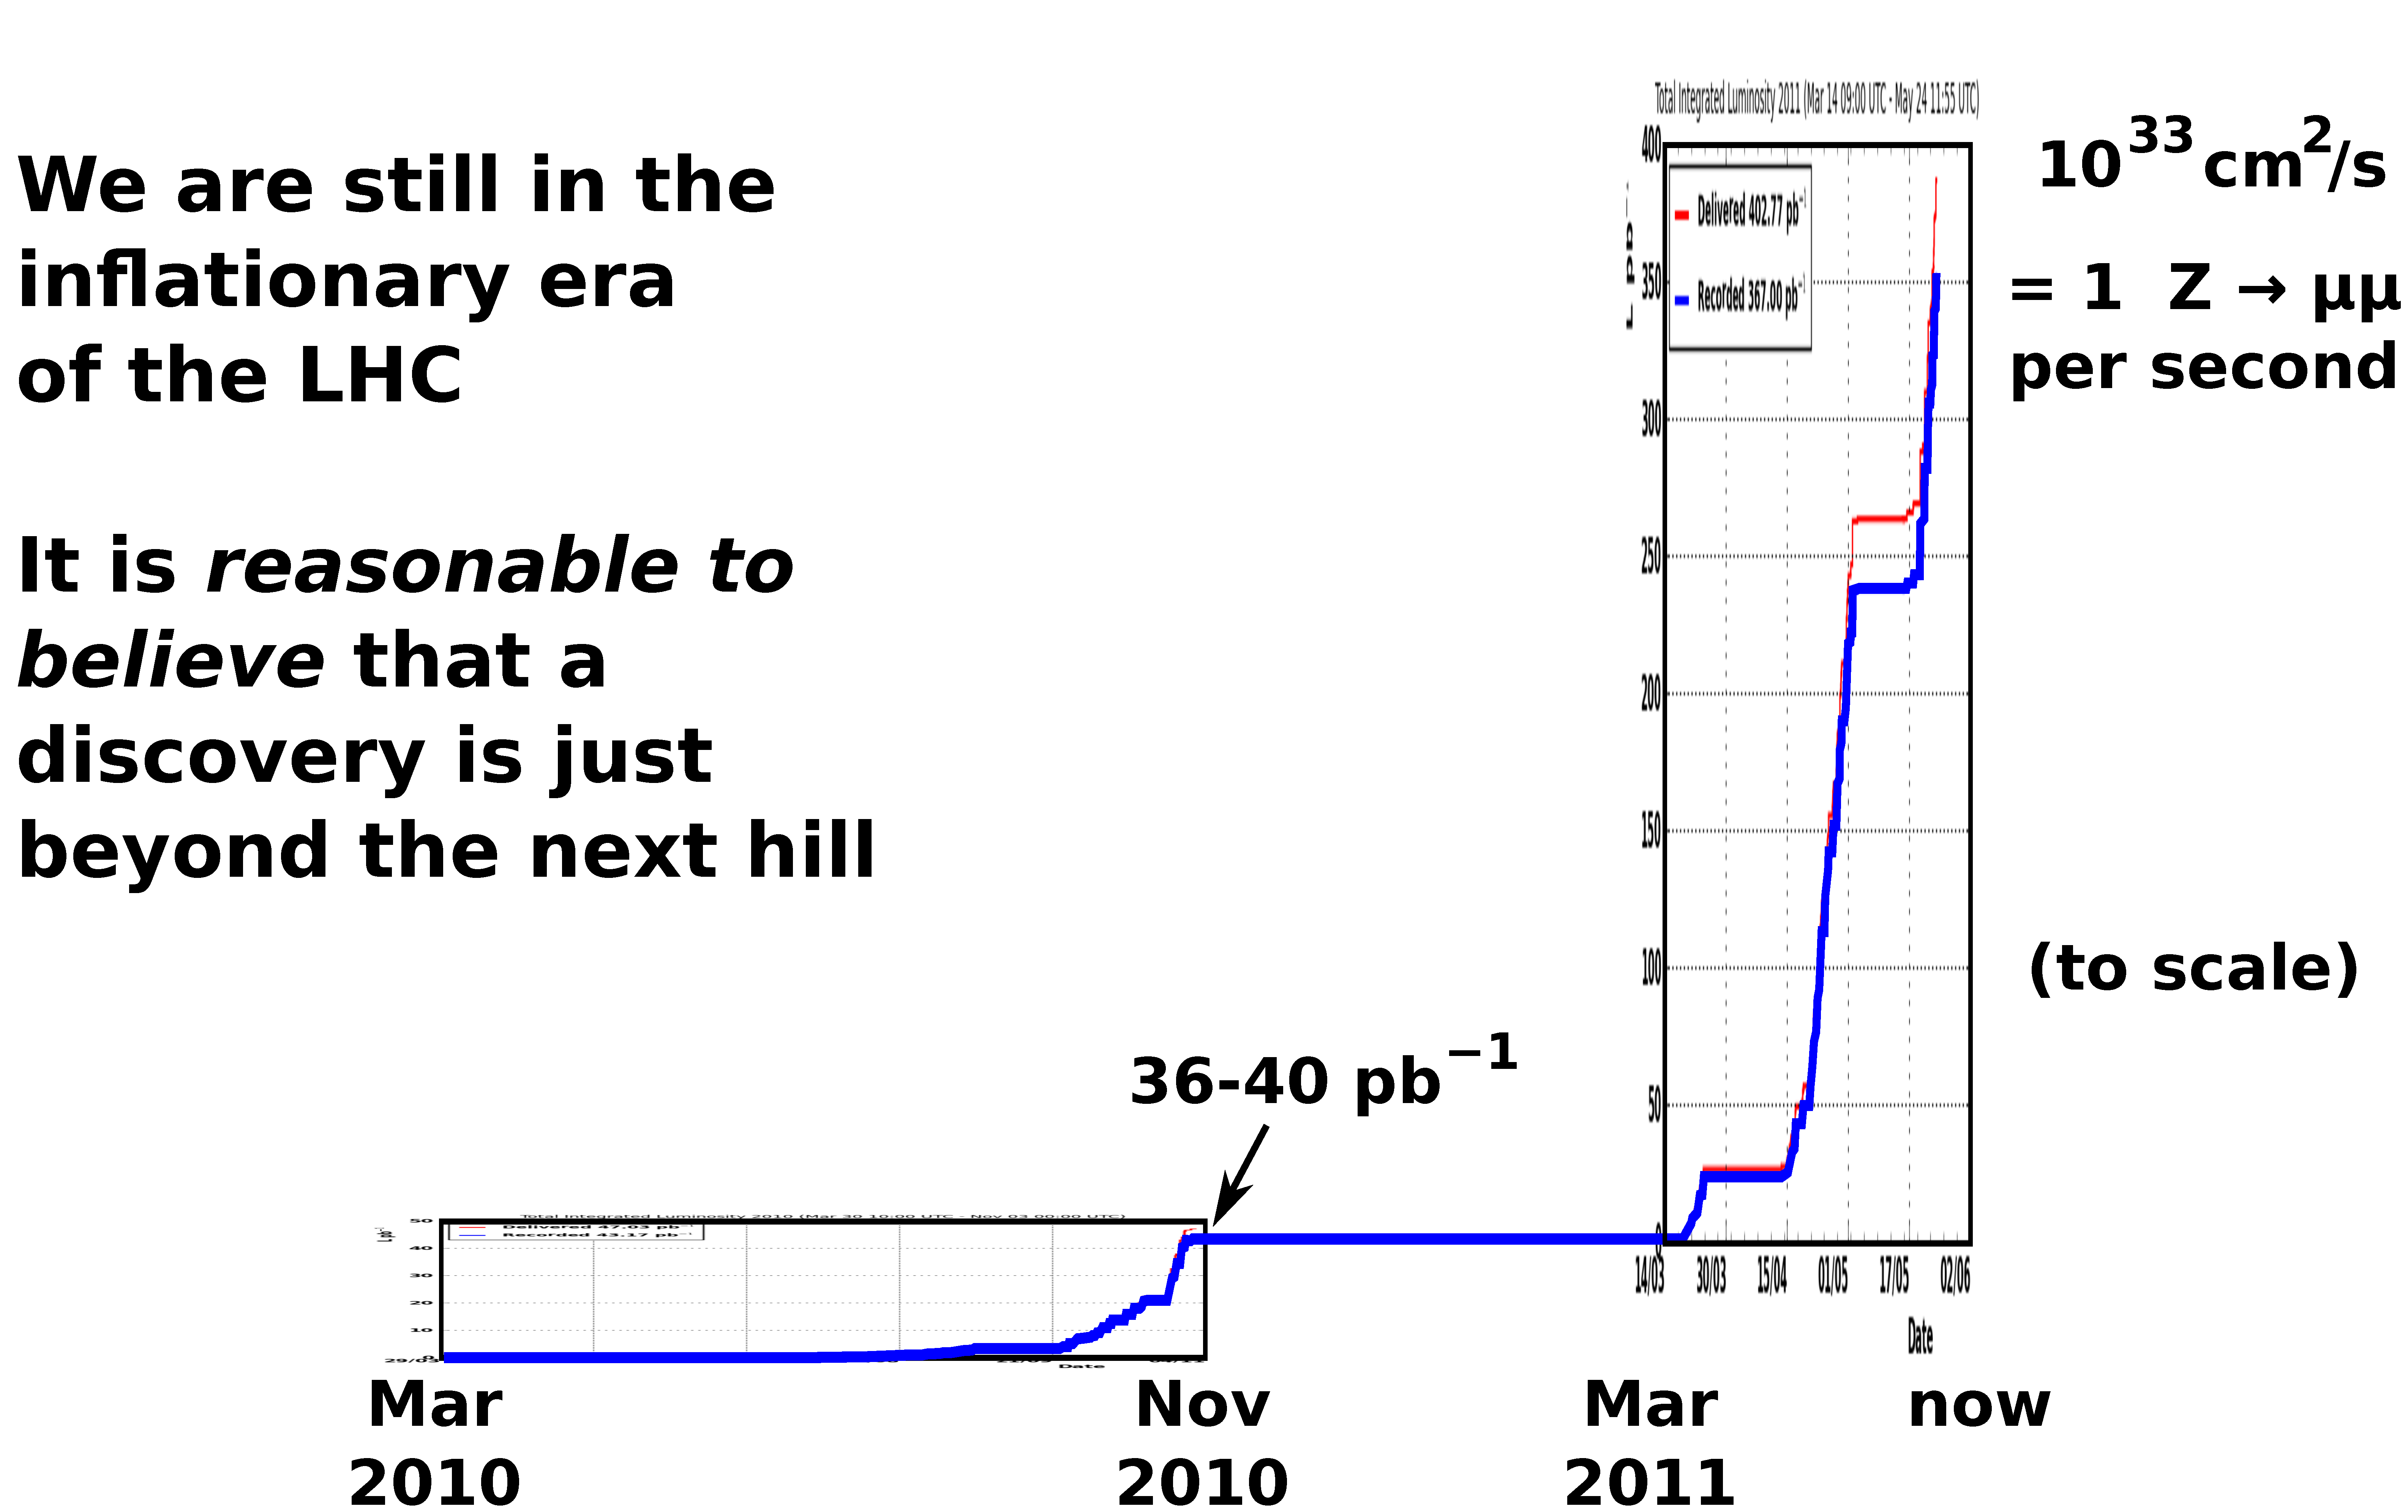
\includegraphics[width=\linewidth]{totallumivstime.pdf}
\end{center}

\textcolor{darkblue}{This talk:} results from the 36-40~pb$^{-1}$ collected in 2010
\end{frame}

\begin{frame}
\frametitle{Ways of presenting search results}

\only<1>{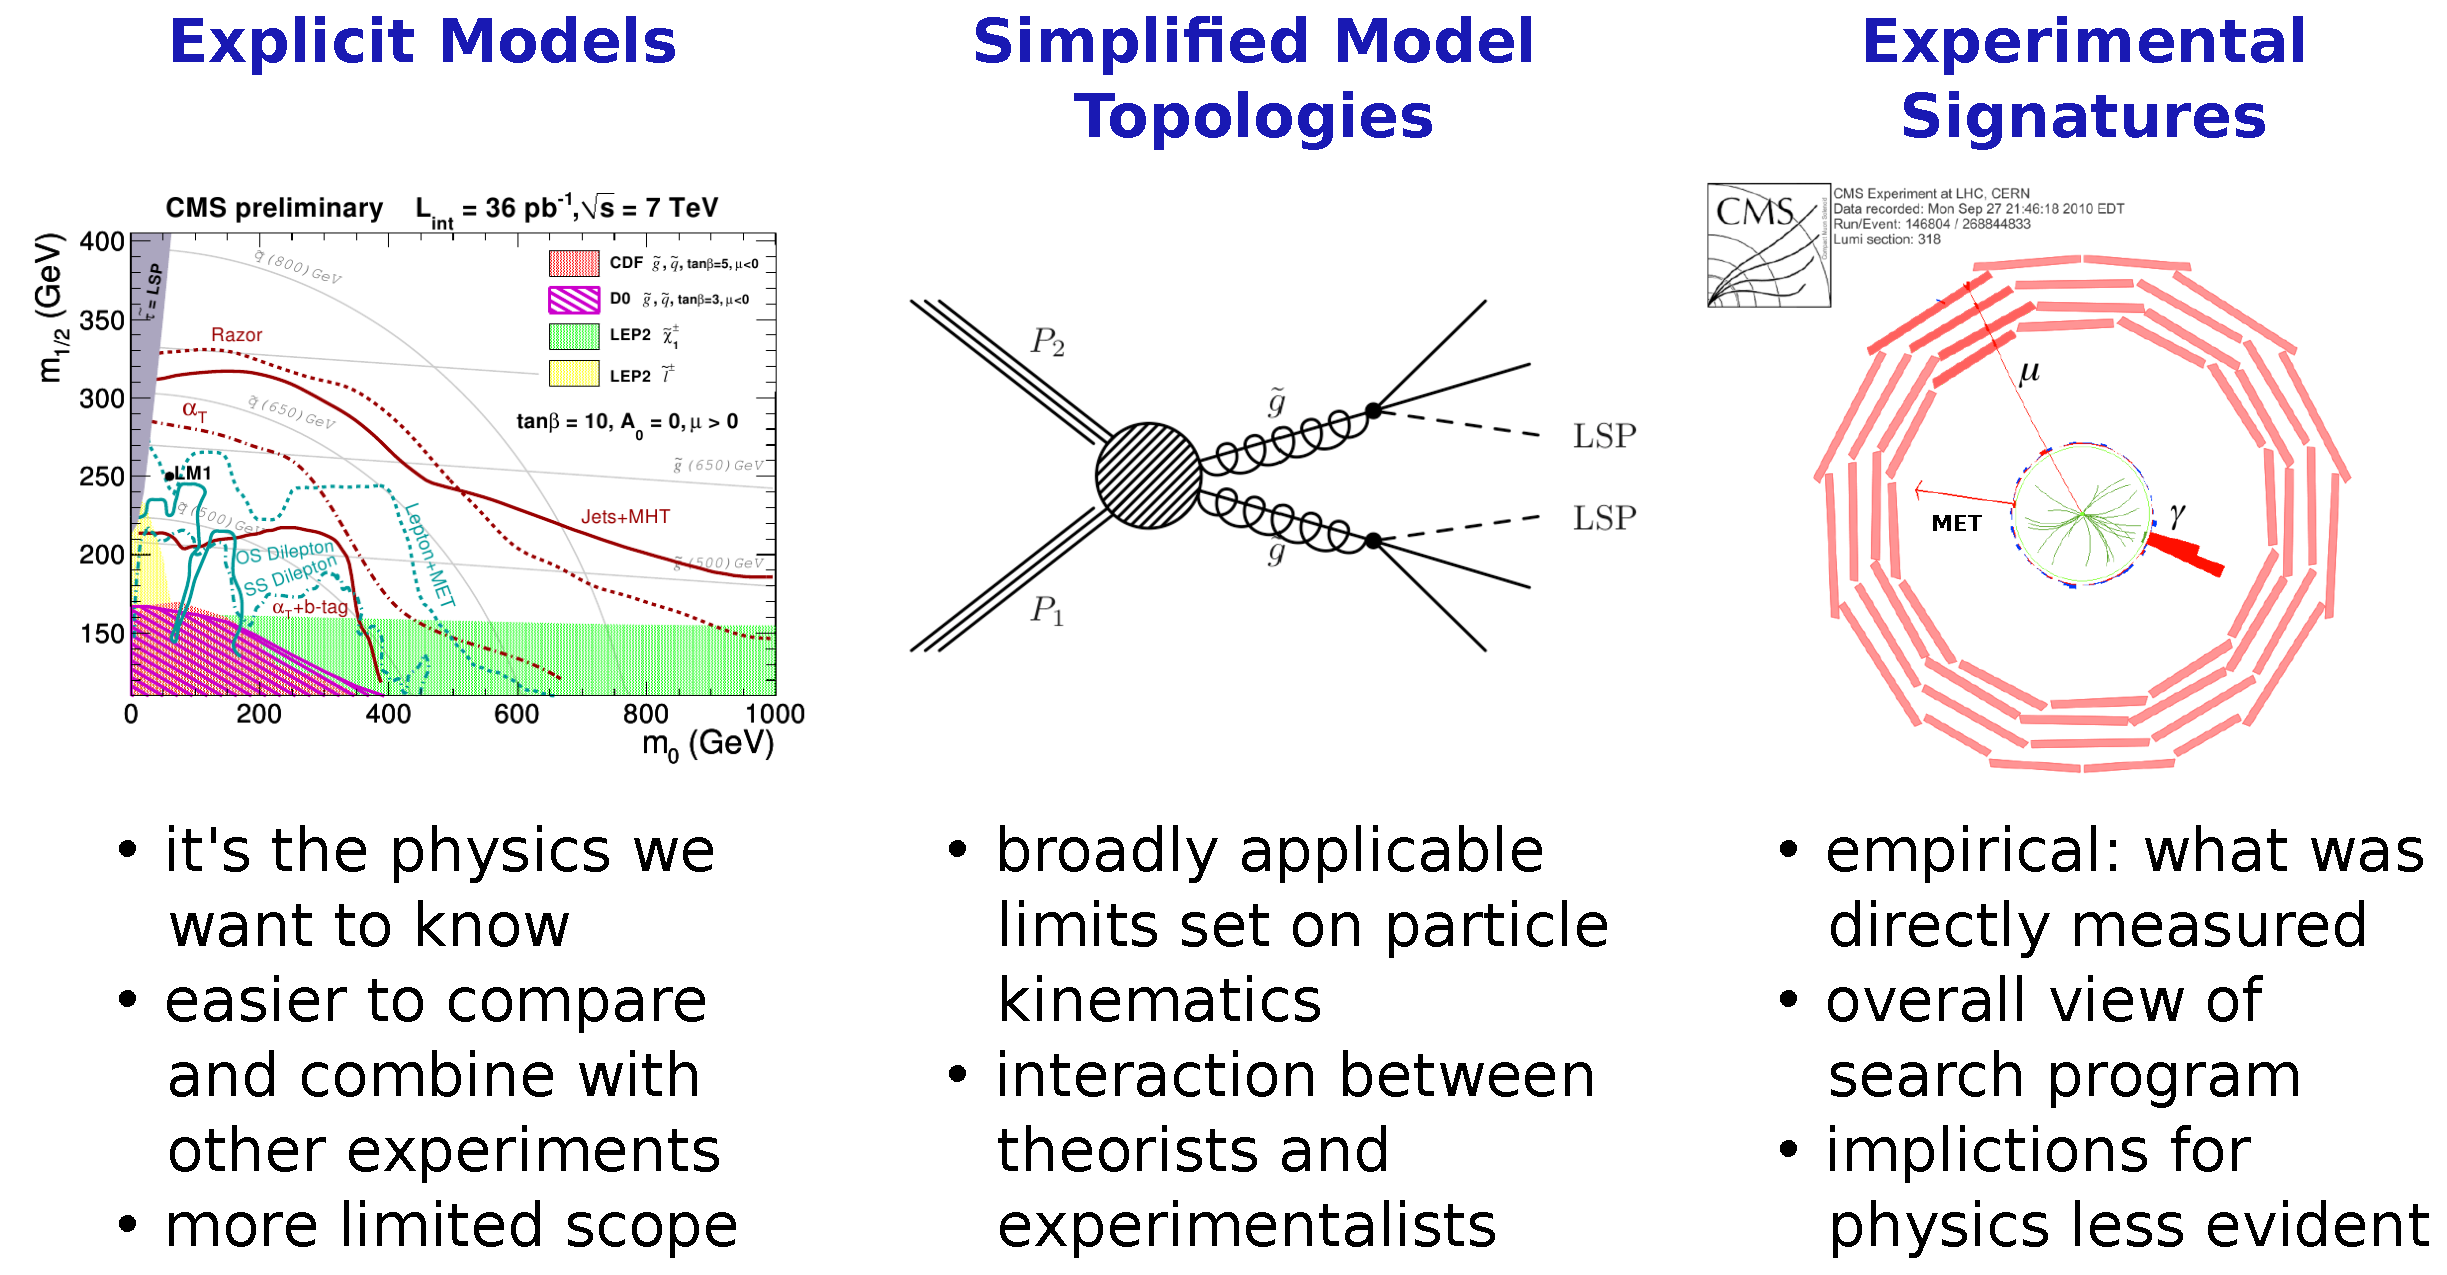
\includegraphics[width=\linewidth]{presentation_styles.pdf}}
\only<2-3>{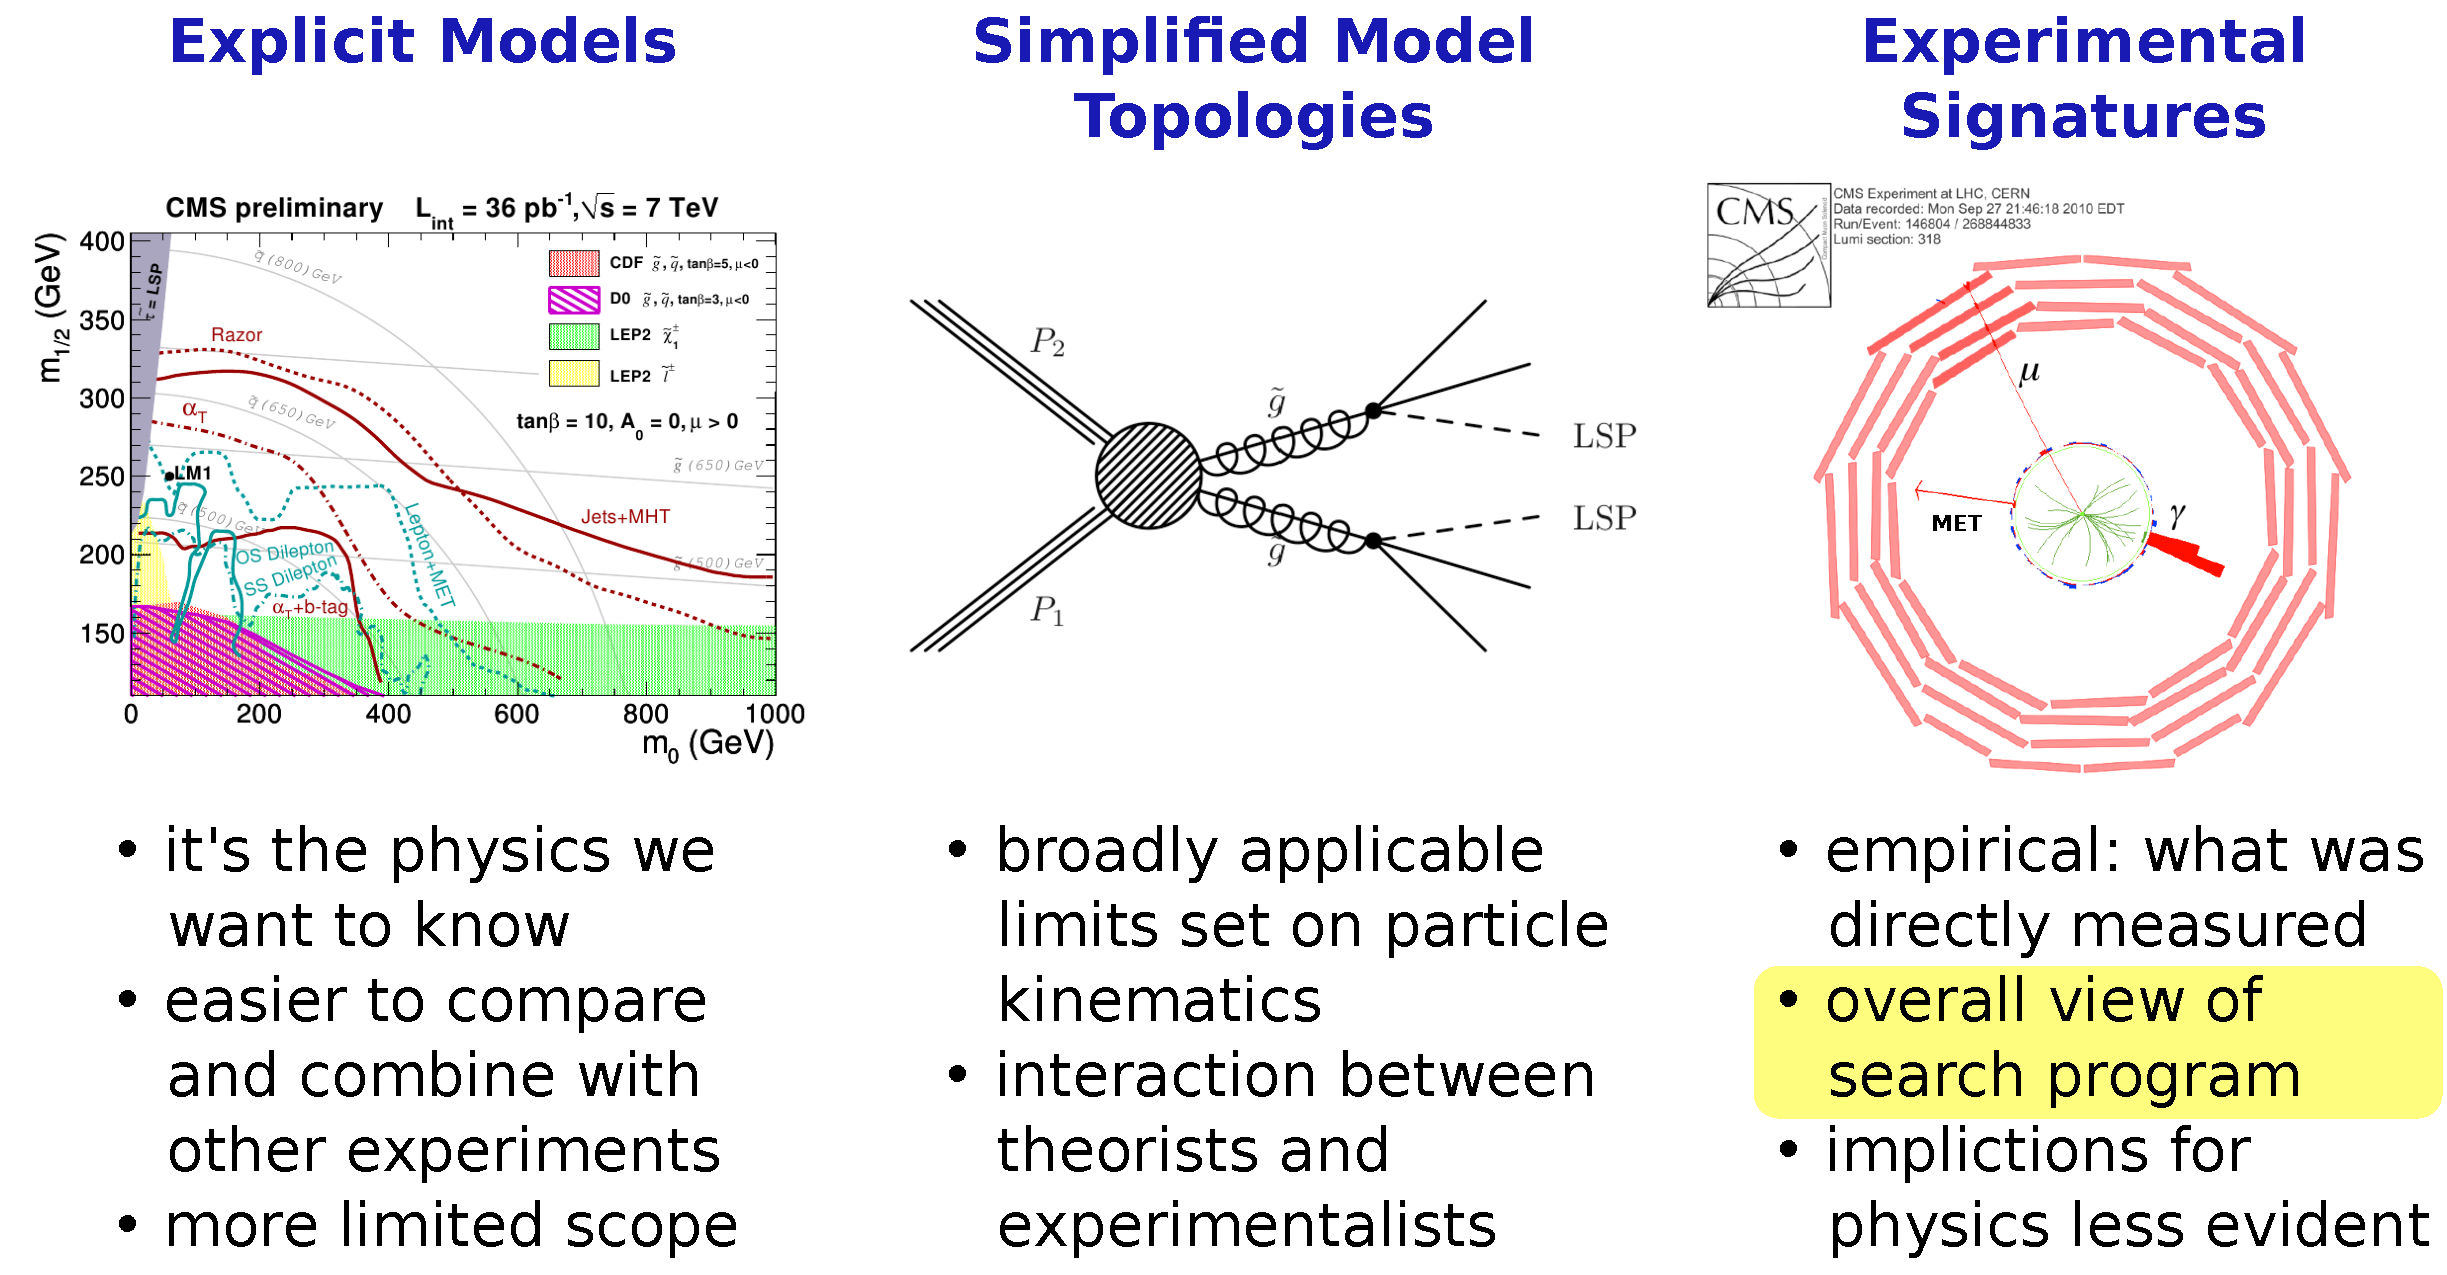
\includegraphics[width=\linewidth]{presentation_styles_2.pdf}}

\begin{itemize}
\item<2-> This talk is organized by experimental signature, for a \mbox{broad overview\hspace{-1 cm}}

\item<3-> For most results, I will show a plot of the experimental channel and point to a paper reference for exact limits and analysis details
\end{itemize}
\end{frame}

\begin{frame}
\frametitle{Outline}
\begin{center}
\begin{minipage}{0.8\linewidth}
\begin{itemize}\setlength{\itemsep}{0.35 cm}
\item Jets and MET
\item Leptons
\item Photons
\item Cross-channels
\item High-level objects ($b$-jets, $\tau$, and top)
\item Weird stuff (e.g.\ new detector signatures)
\end{itemize}
\end{minipage}
\end{center}

\end{frame}

\begin{frame}
\frametitle{Jets: resonances}

\begin{columns}
\column{0.3\linewidth}

Generic searches for hadronic resonances

\textcolor{darkblue}{\scriptsize dijet: hep-ex/1010.0203}
\begin{itemize}
\item $Z'$ or $G^* \to q\bar{q}$
\end{itemize}

\textcolor{darkblue}{\scriptsize \mbox{multijet: PAS EXO-11-001\hspace{-1 cm}}}
\begin{itemize}
\item ``quix'' or {\scriptsize RPV}~$\tilde{g}$ \\ \hfill $\to qq\bar{q}$
\end{itemize}

\column{0.7\linewidth}
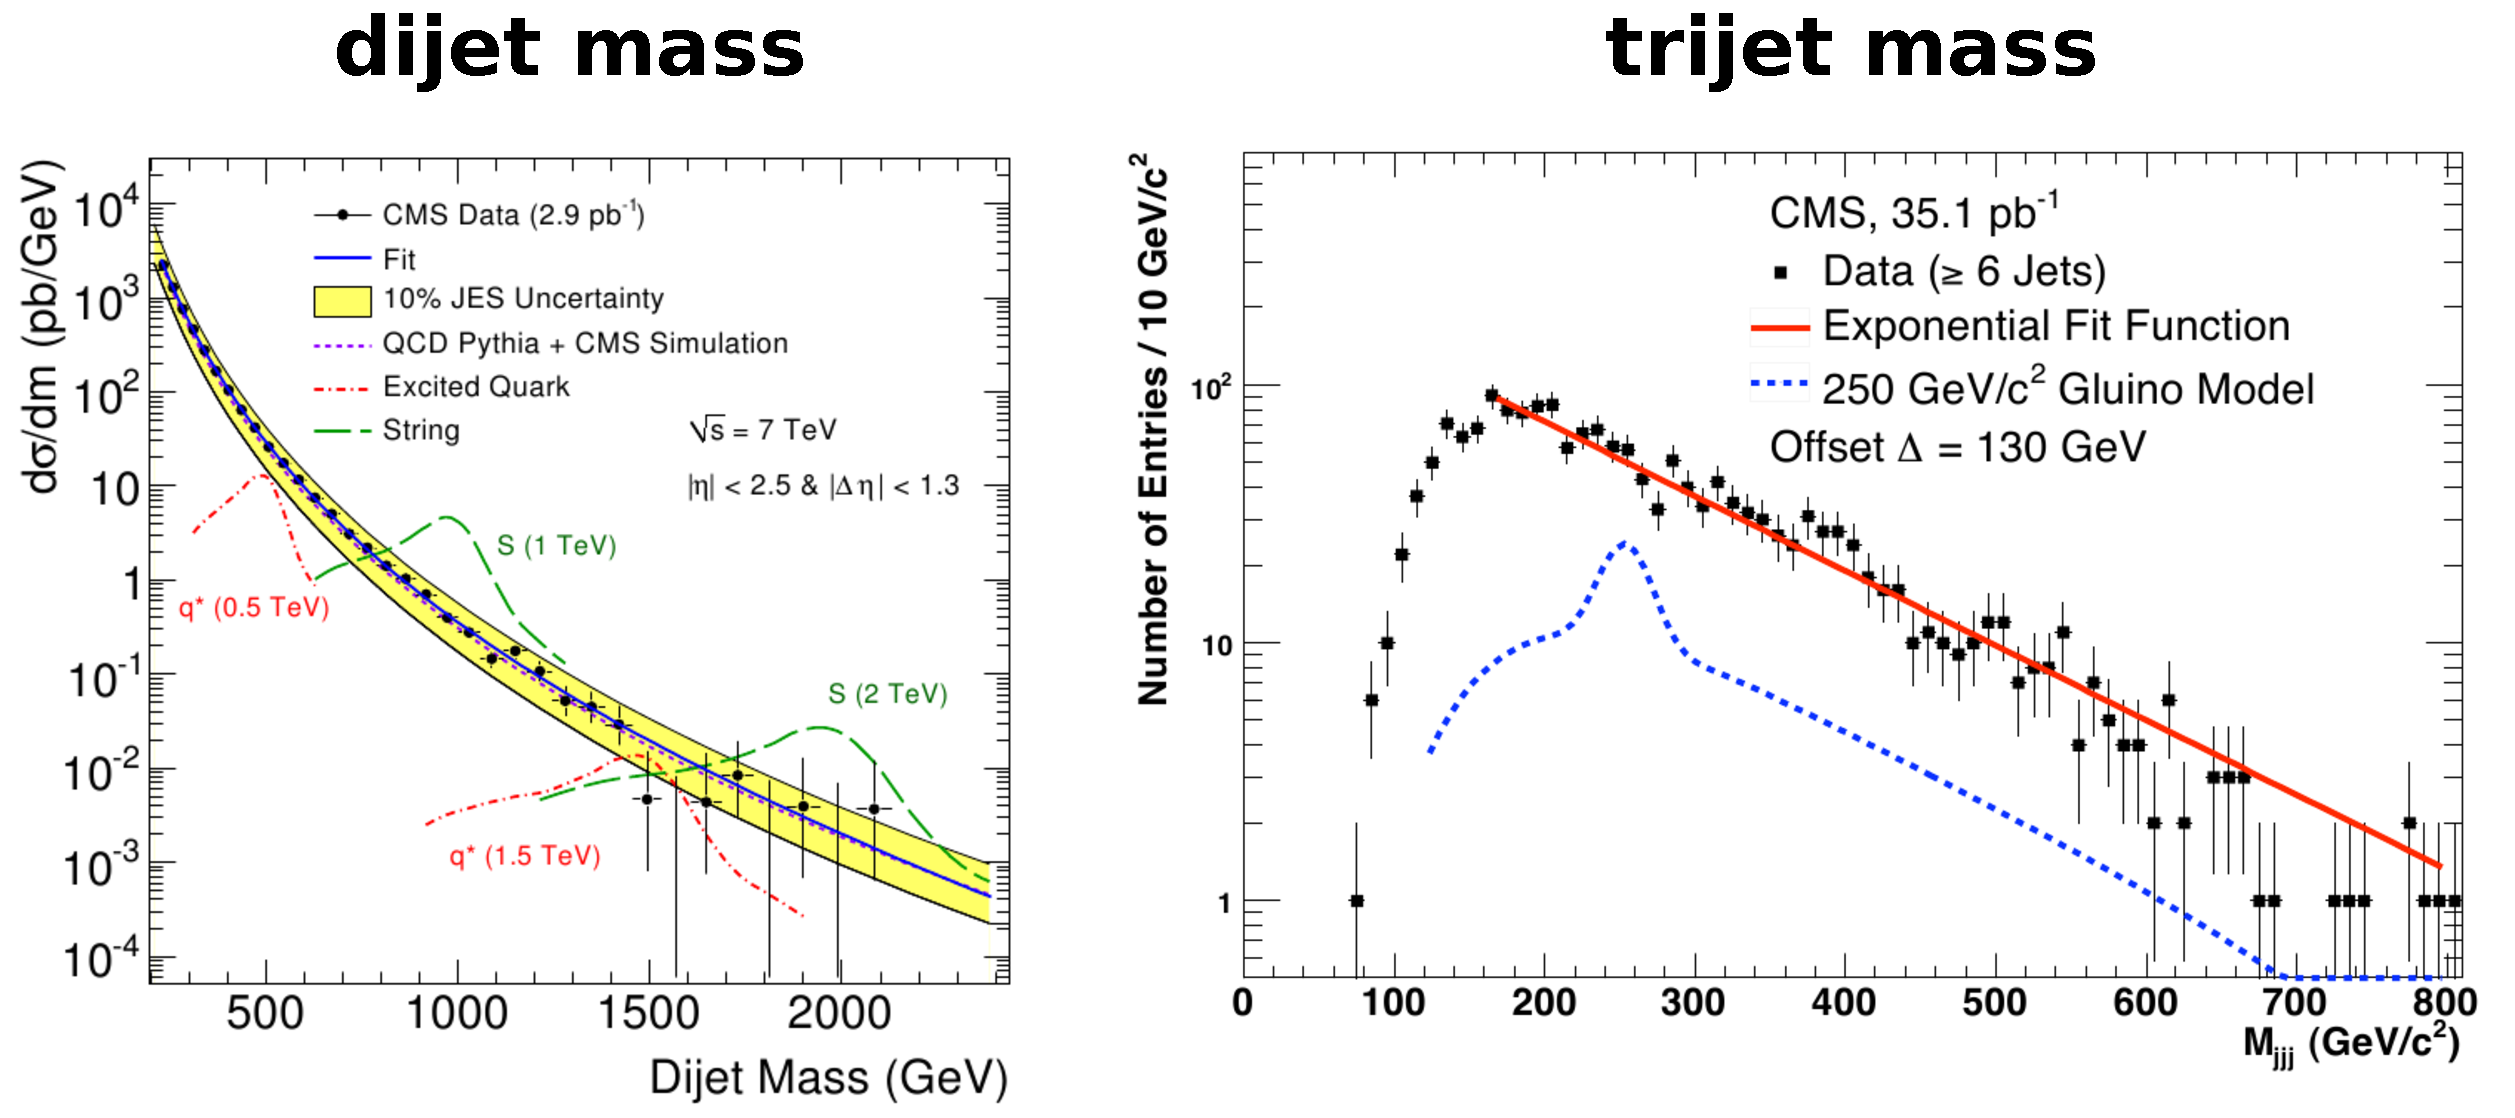
\includegraphics[width=\linewidth]{figures/dijet_trijet.pdf}
\end{columns}

\vfill
\uncover<2->{\hspace{-0.83 cm} \textcolor{darkblue}{\Large Dijet angular distributions}
\begin{columns}
\column{0.65\linewidth}

\vspace{0.3 cm}
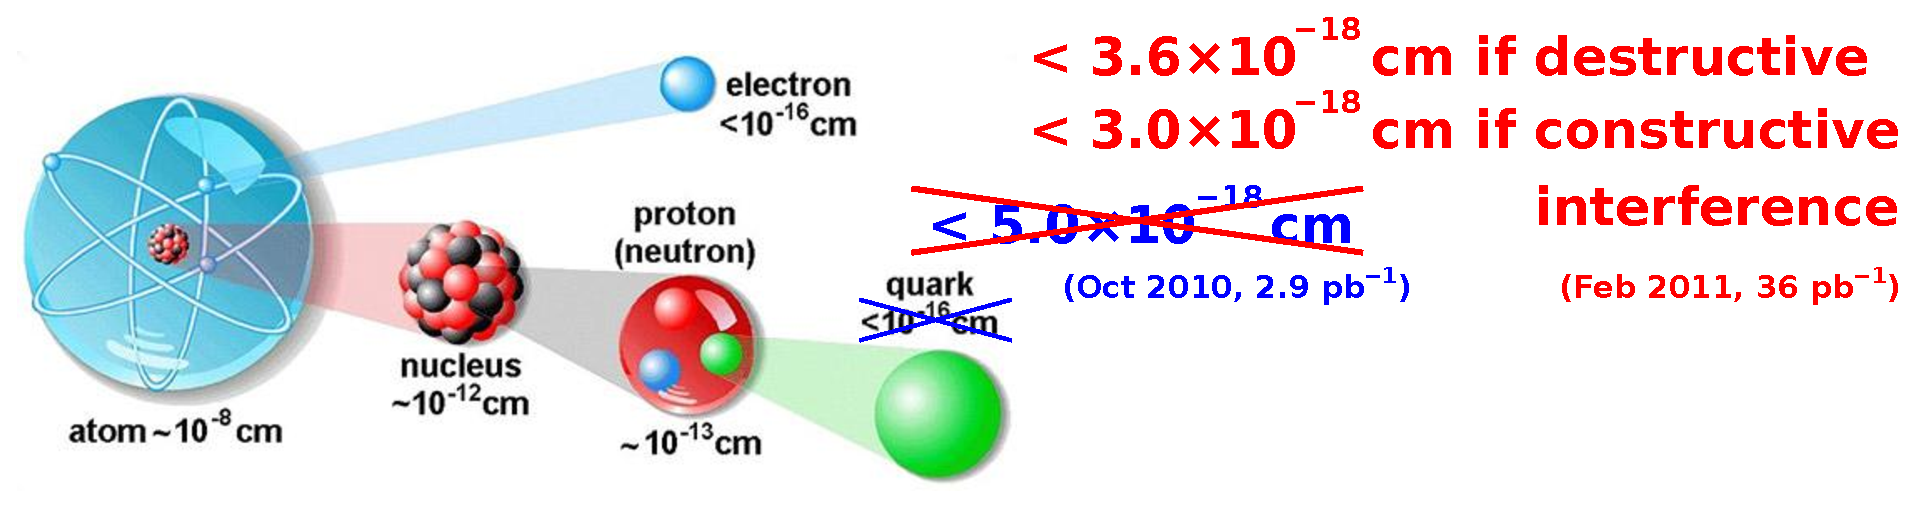
\includegraphics[width=\linewidth]{figures/atom_zoom_b.pdf}

\vspace{0.3 cm}
\textcolor{darkblue}{\scriptsize hep-ex/1010.4439 \textcolor{black}{and} hep-ex/1102.2020 (update)}

\column{0.35\linewidth}

\vspace{-0.6 cm}
Centrality ratio

\vspace{0.1 cm}
\mbox{$\displaystyle R_\eta = \frac{N_{jj}(|\eta| < 0.7)}{N_{jj}(0.7 < |\eta| < 1.3)}$}

\vspace{0.1 cm}
New limits on quark compositeness:

\vspace{0.1 cm}
\hspace{0.25 cm} $\Lambda^+ > 5.6$~TeV \mbox{\scriptsize (destr.)\hspace{-1 cm}}

\hspace{0.25 cm} $\Lambda^- > 6.7$~TeV \mbox{\scriptsize (constr.)\hspace{-1 cm}}
\end{columns}}
\end{frame}

\begin{frame}
\frametitle{SUSY jets: special variables}

\vspace{0.4 cm}
\begin{columns}
\column{0.33\linewidth}

\vspace{-0.4 cm}
$\alpha_T = p_{T2}/M_T$ where $p_{T2}$ is the second-highest jet momentum

\vspace{0.2 cm}
Only events with real MET have $\alpha_T > 0.55$

\textcolor{darkblue}{\scriptsize hep-ex/1101.1628 \textcolor{black}{and} PAS~SUS-11-001}

\column{0.33\linewidth}
\scriptsize \centering $H_T > 350$~GeV dijets

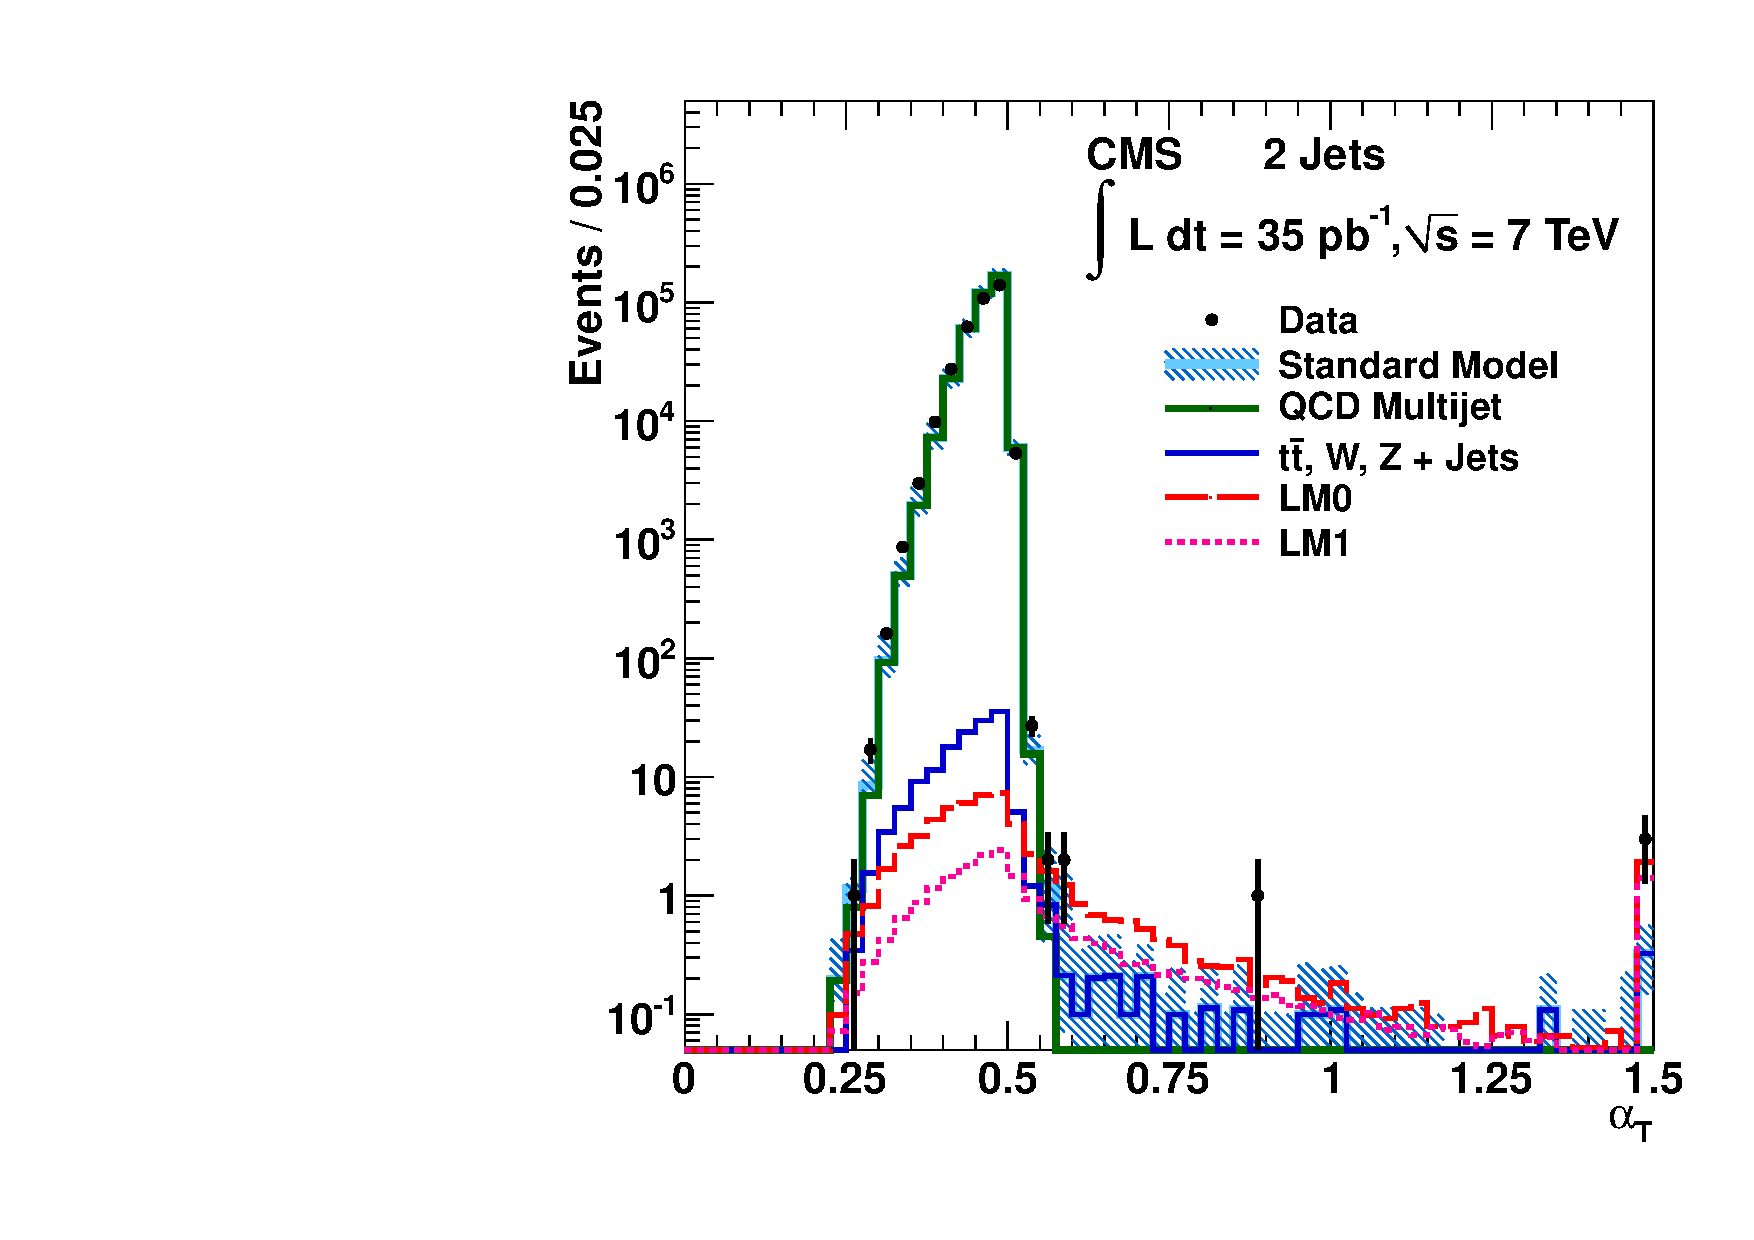
\includegraphics[width=\linewidth]{plots/alphat_dijets.pdf}

\column{0.33\linewidth}
\scriptsize \centering $H_T > 350$~GeV multijets

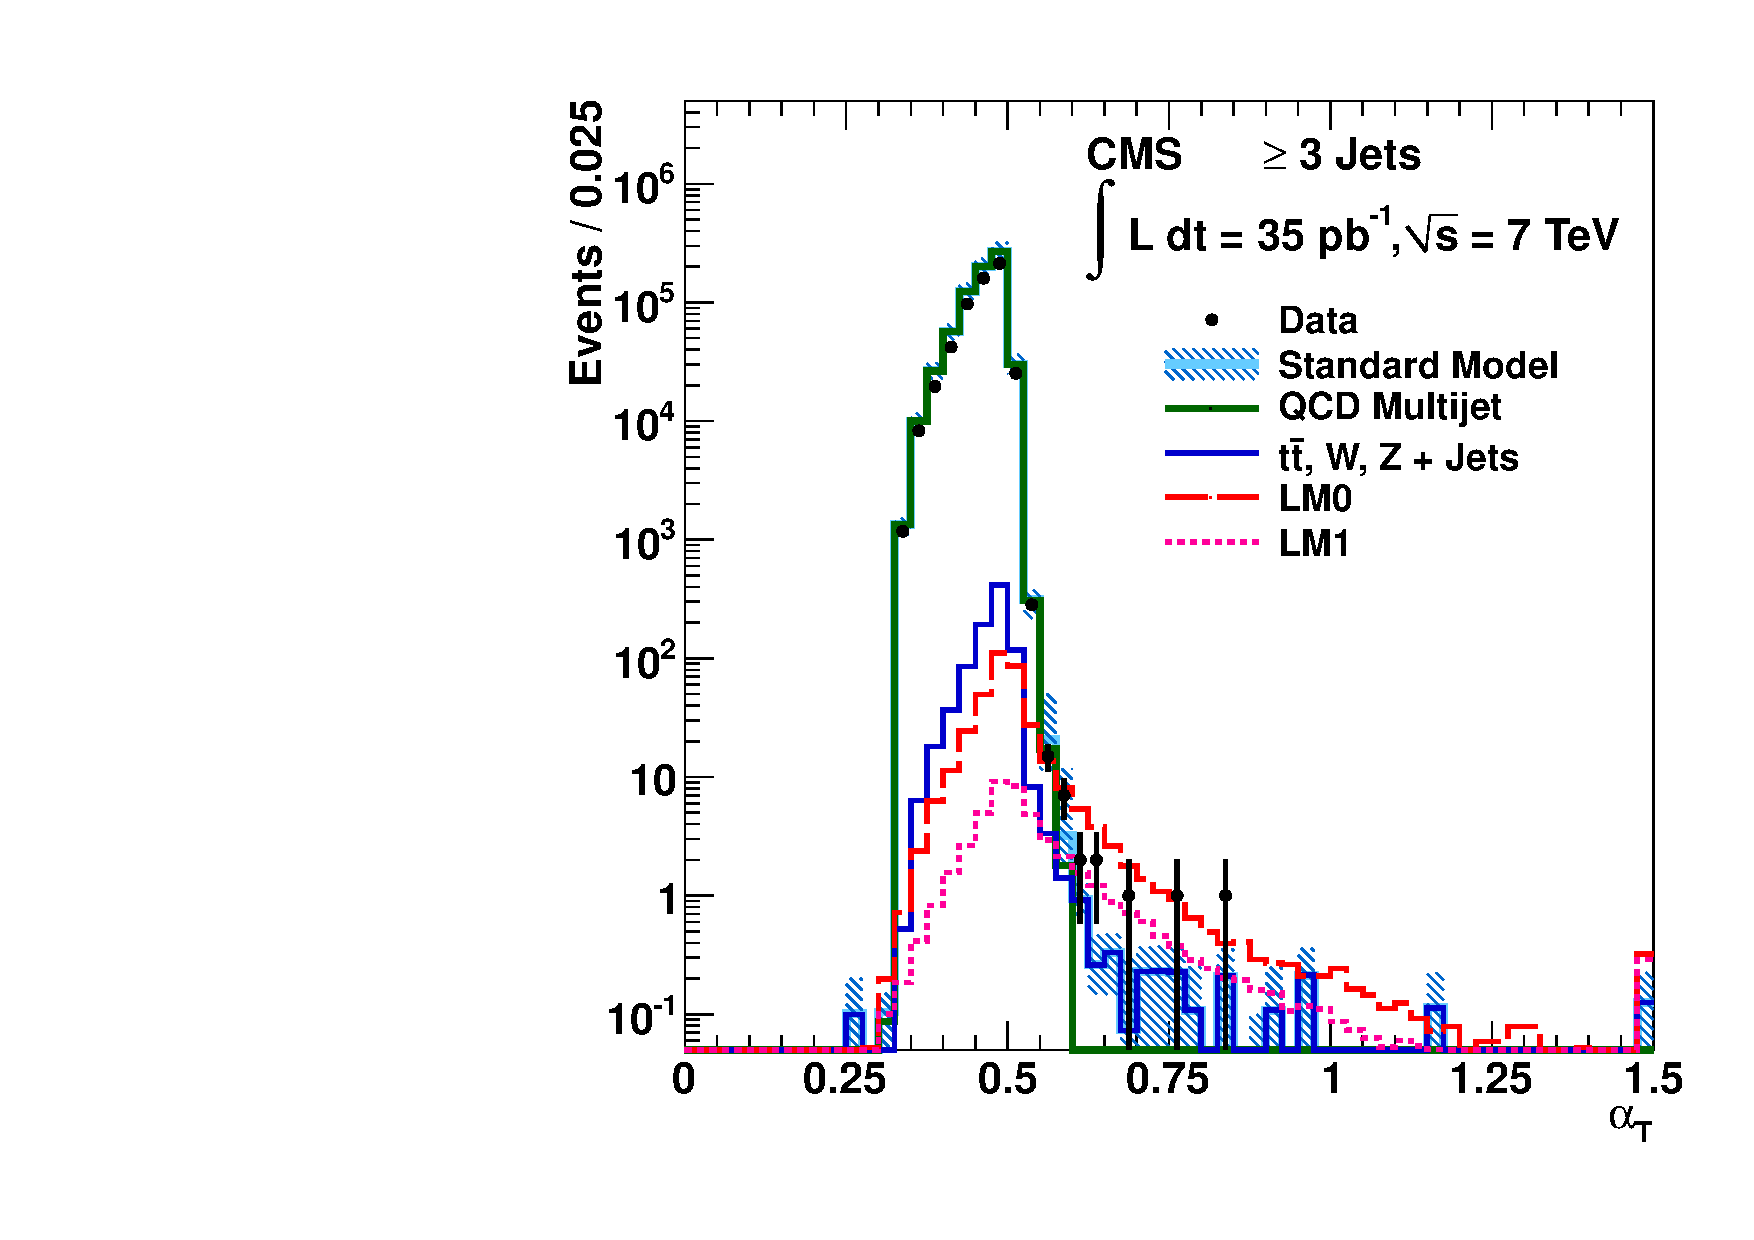
\includegraphics[width=\linewidth]{plots/alphat_multijets.pdf}
\end{columns}

\uncover<2->{\begin{columns}
\column{0.5\linewidth}
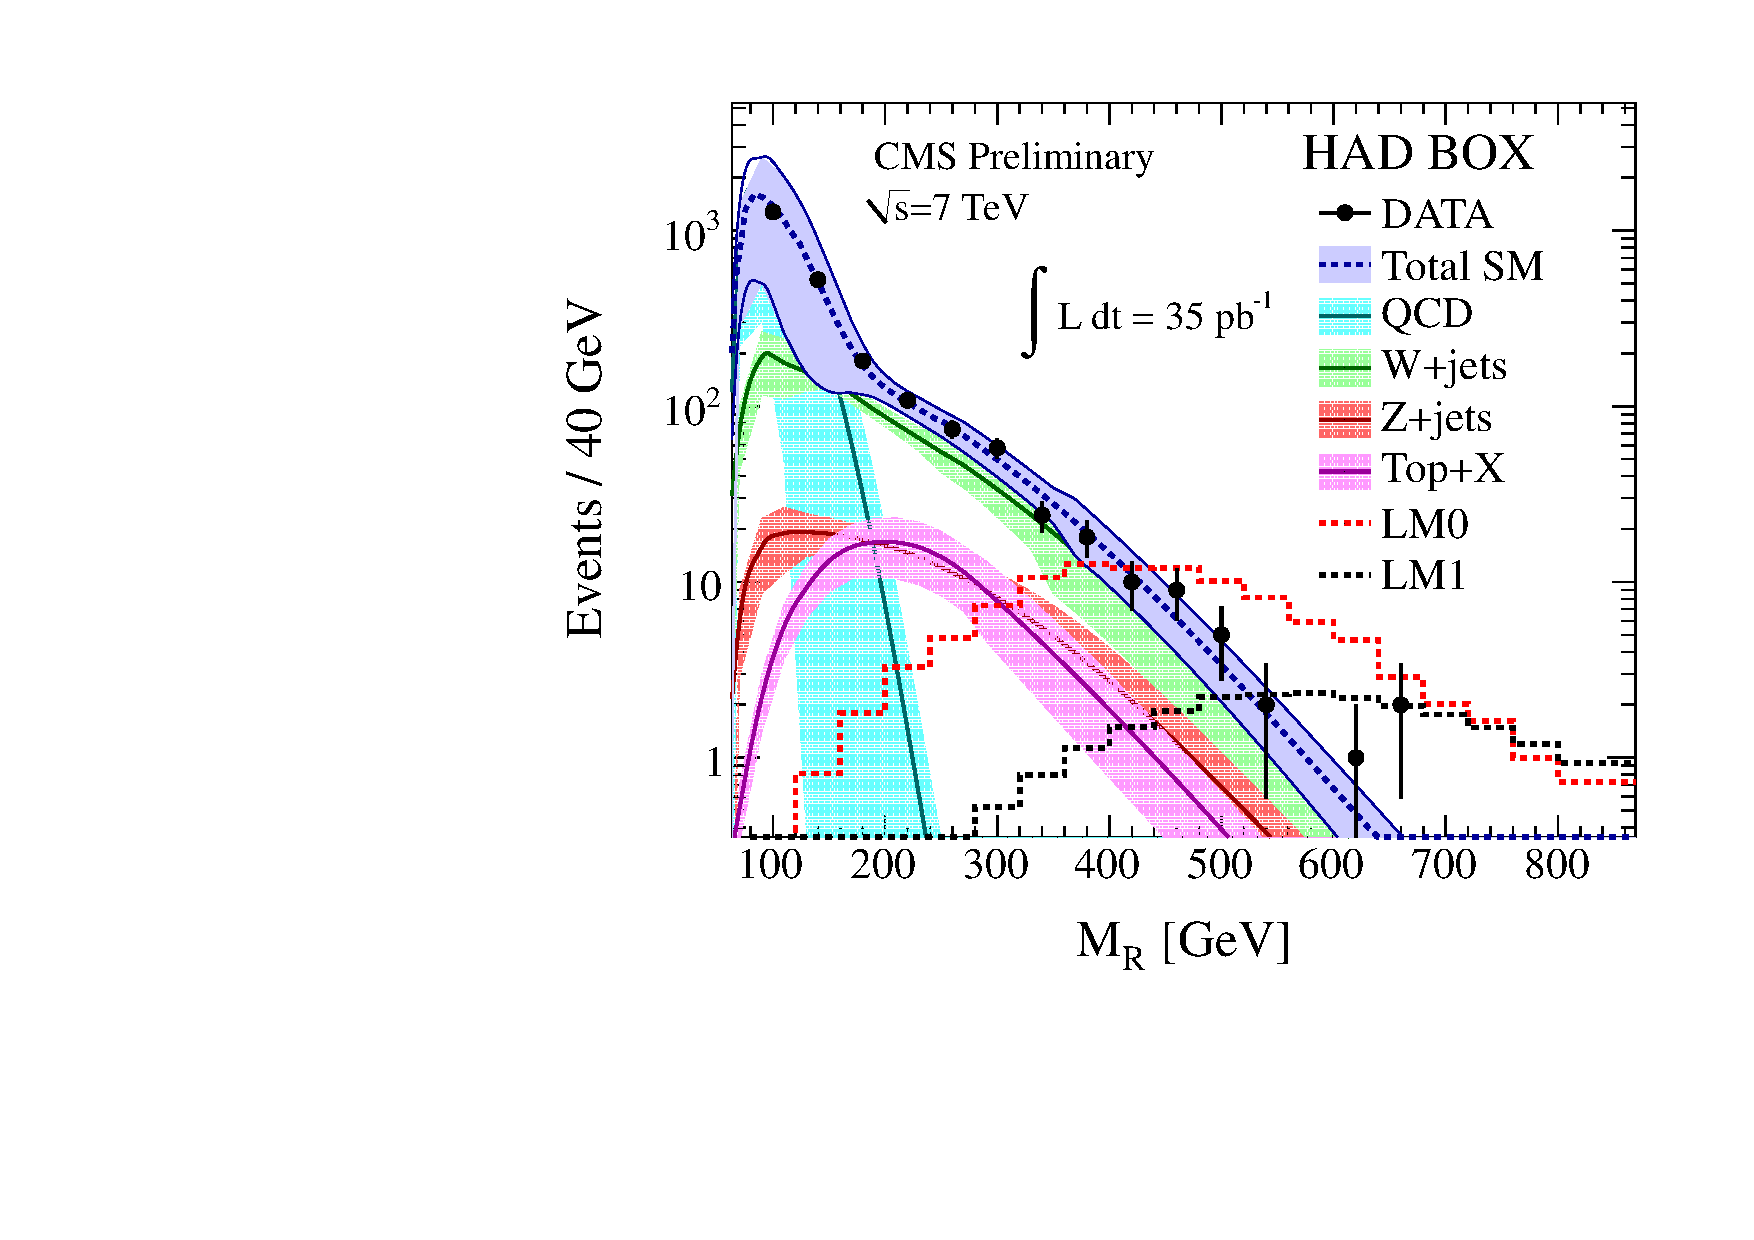
\includegraphics[width=\linewidth]{plots/mr_razor.pdf}

\column{0.5\linewidth}
``Razor'' analysis:

\vspace{-0.2 cm}
\begin{itemize}\setlength{\itemsep}{-0.1 cm}
\item interpret event as decay of two heavy objects: $pp \to MM$
\item split jet activity into hemispheres; $M_R =$ hemisphere momentum in boosted frame
\item $R = M^R_T/M_R$, \mbox{search in $R > 0.5$\hspace{-1 cm}}
\end{itemize}

\hfill \textcolor{darkblue}{\scriptsize PAS SUS-10-009}
\end{columns}}
\end{frame}

\begin{frame}
\frametitle{SUSY jets: simplified models}

\begin{itemize}
\item Inclusive search for new physics in $\ge 3$ jets and missing energy

\hfill \textcolor{darkblue}{\scriptsize (PAS SUS-10-005)}

\item Results expressed as limits on cMSSM and simplified models (below)

\item Data file provided with acceptances, uncertainties, and limits as a function of simplified model particle masses
\end{itemize}

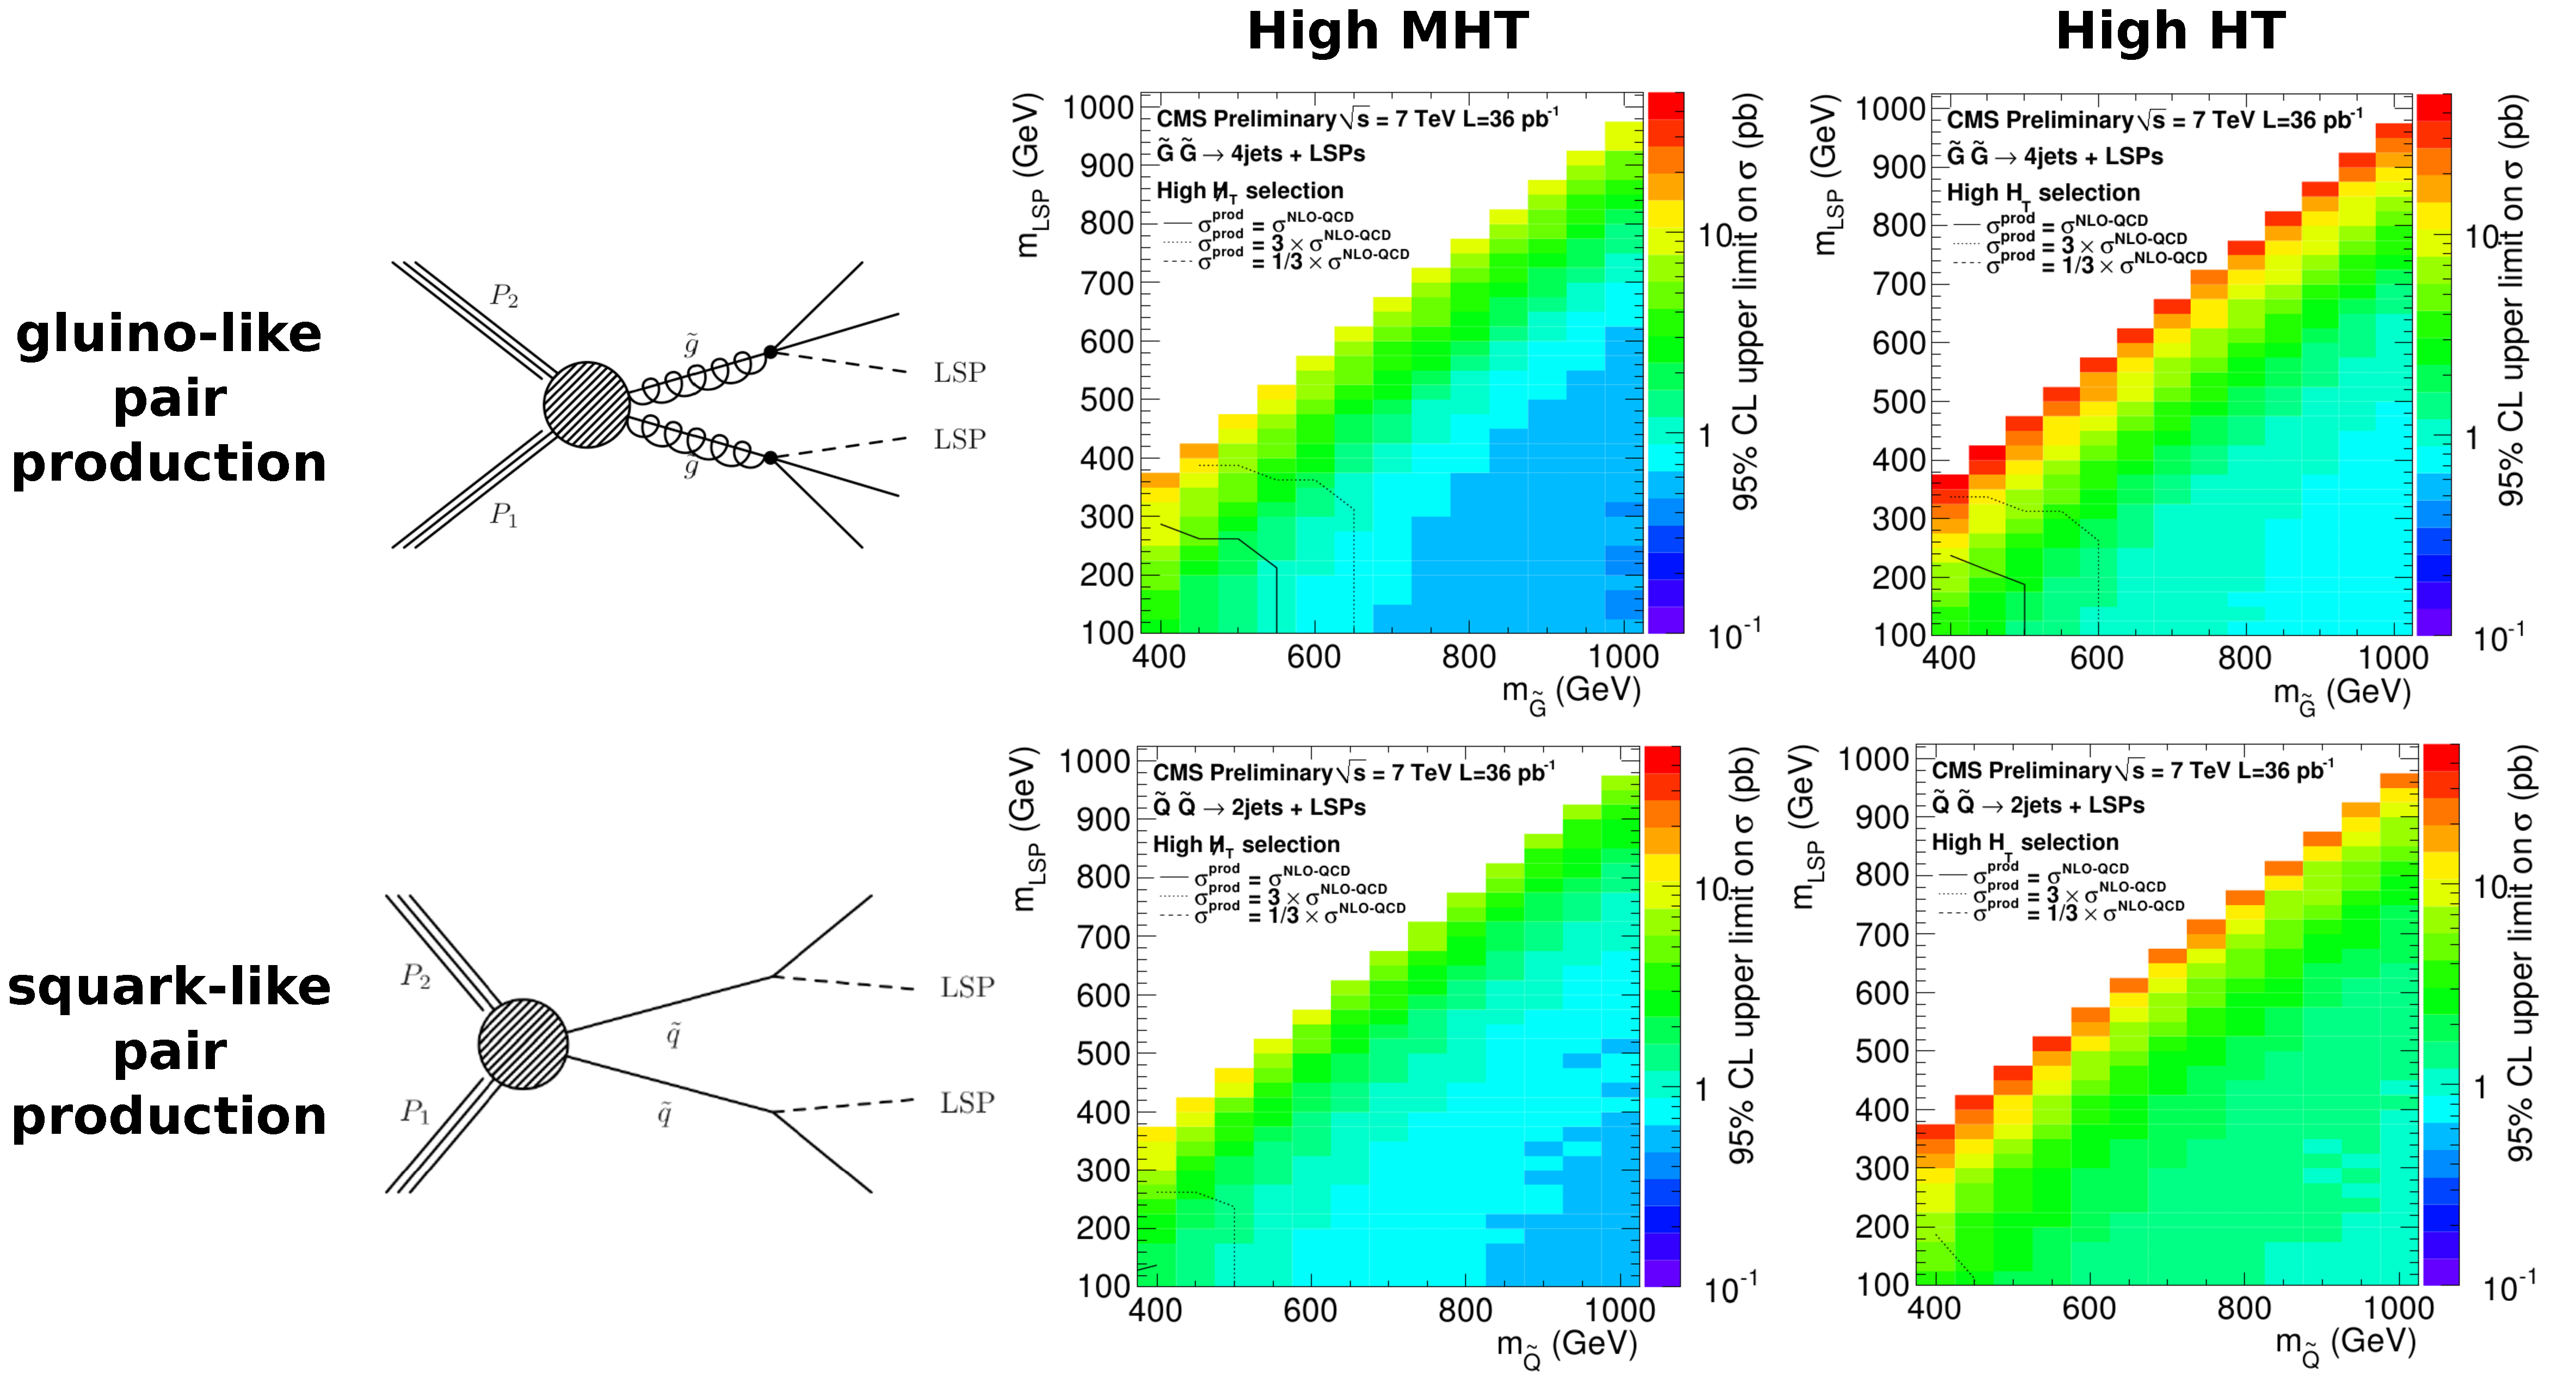
\includegraphics[width=\linewidth]{plots/sms_plots.pdf}
\end{frame}

\begin{frame}
\frametitle{Leptons}

\begin{columns}
\column{0.4\linewidth}
\begin{itemize}
\item Dilepton resonances: \\ several kinematic regions for searches
\end{itemize}

\vspace{1 cm}

\column{0.68\linewidth}
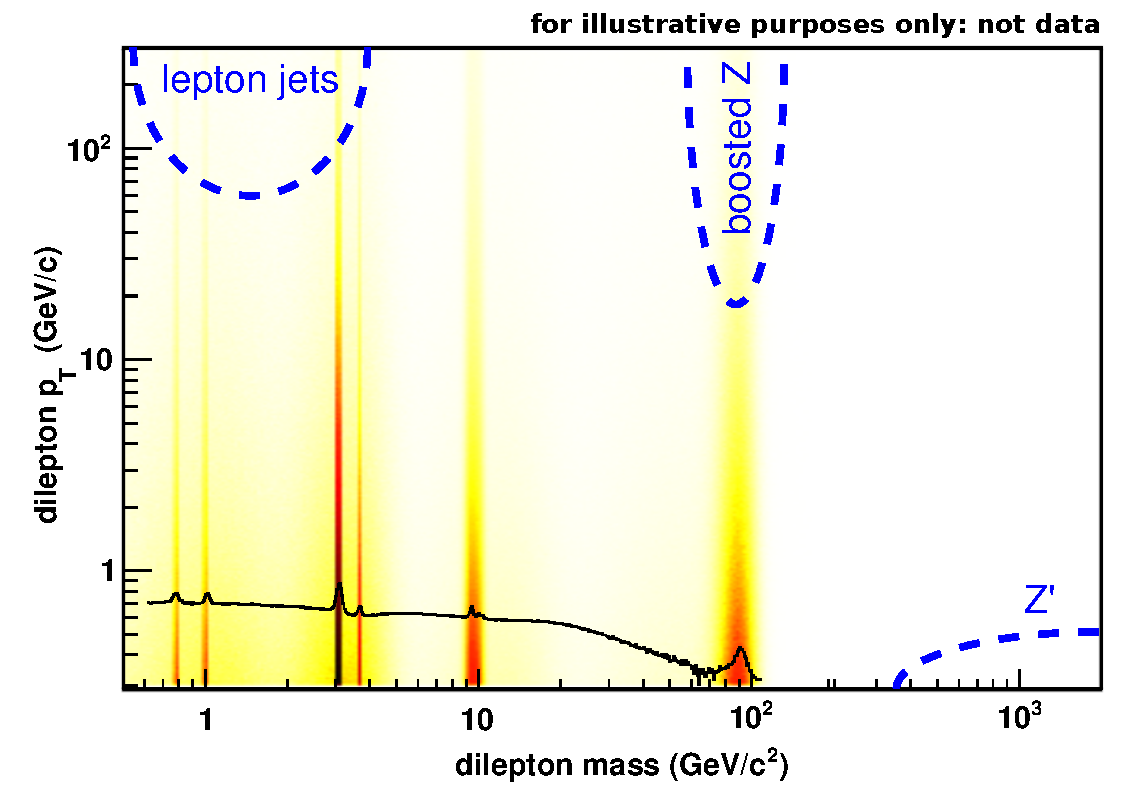
\includegraphics[width=\linewidth]{figures/spectrum_mumu.pdf}
\end{columns}

\begin{columns}
\column{0.4\linewidth}
\uncover<2->{\begin{minipage}{1.25\linewidth}
\begin{itemize}
\item Other exotica searches
\begin{itemize}
\item non-resonant dimuons: large extra dimensions

\hfill \textcolor{darkblue}{\scriptsize PAS EXO-10-020}

\item high muon multiplicity: lepton jets
\end{itemize}
\end{itemize}
\end{minipage}}

\column{0.65\linewidth}
\uncover<3->{\begin{minipage}{\linewidth}
\begin{itemize}
\item SUSY searches
\begin{itemize}
\item single lepton \hfill \textcolor{darkblue}{\scriptsize SUS-10-006}
\item opp-sign dilepton \hfill \textcolor{darkblue}{\scriptsize hep-ex/1103.1348}
\item same-sign dilepton \hfill \textcolor{darkblue}{\scriptsize hep-ex/1104.3168}
\item $\ge 3$ leptons \hfill \textcolor{darkblue}{\scriptsize SUS-10-008} \\ \mbox{ }
\end{itemize}
\end{itemize}
\end{minipage}}
\end{columns}
\end{frame}

\begin{frame}
\frametitle{Leptons: high-mass resonances}

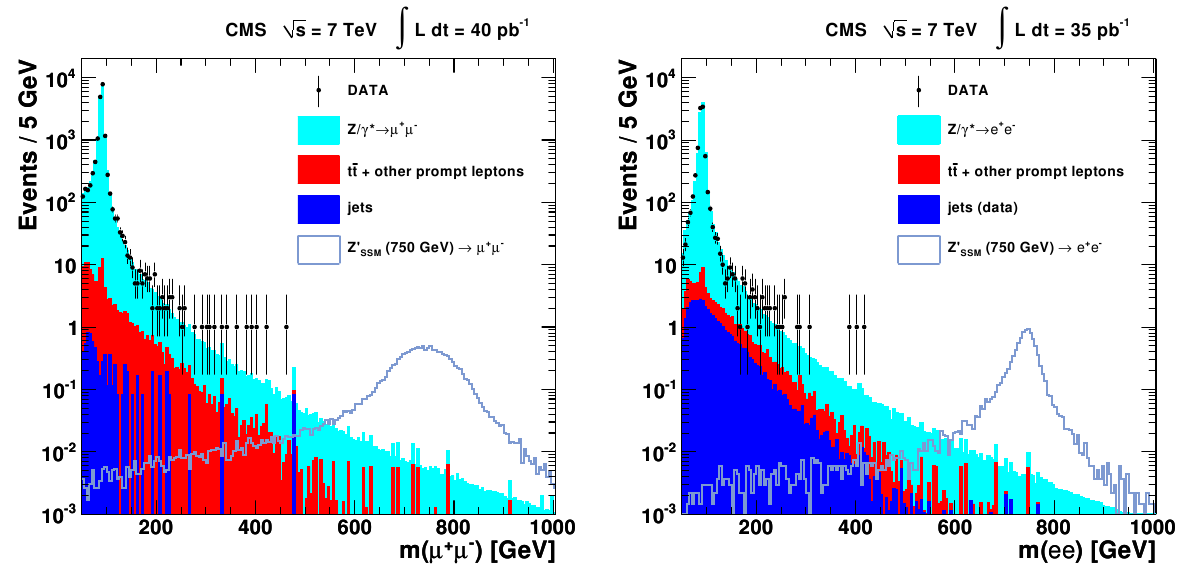
\includegraphics[width=0.75\linewidth]{plots/dilepton_mass.png}

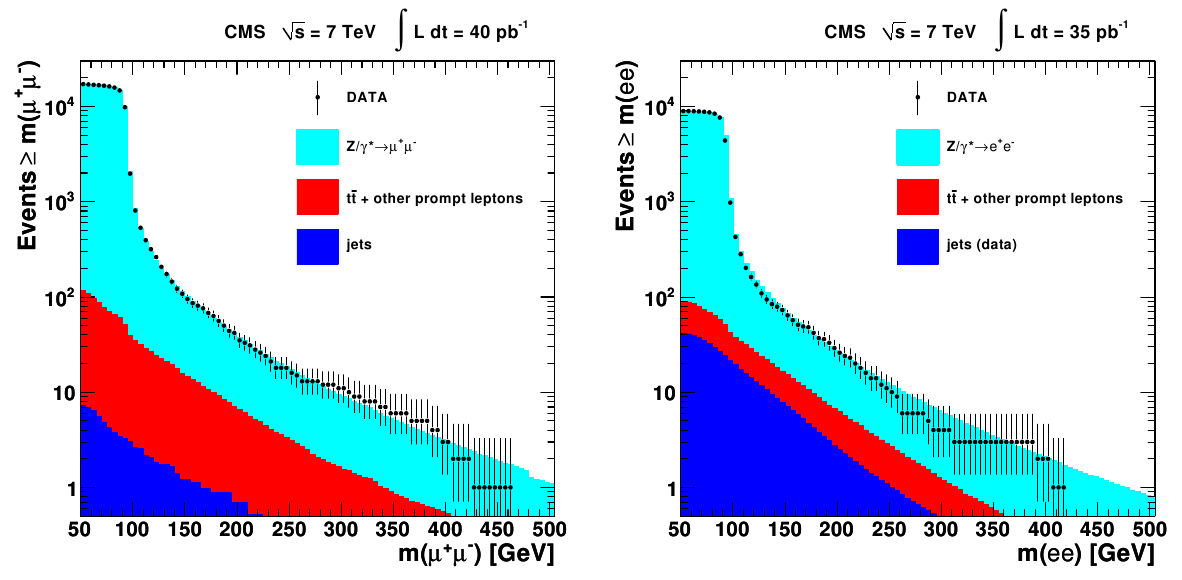
\includegraphics[width=0.75\linewidth]{plots/dilepton_cumulative.png}

\vspace{-1 cm}
\hfill \textcolor{darkblue}{\scriptsize hep-ex/1103.0981}
\end{frame}

\begin{frame}
\frametitle{Leptons: other resonances}

\begin{columns}
\column{0.33\linewidth}
\textcolor{darkblue}{$Z$ boson $p_T$ spectrum:}

channel for generic neutral heavy-to-light decays, e.g.

\mbox{ } \hfill $q^* \to q \, Z$ \hfill \mbox{ }

\vspace{0.1 cm}
\textcolor{darkblue}{\scriptsize PAS EXO 10-025}

\column{0.33\linewidth}
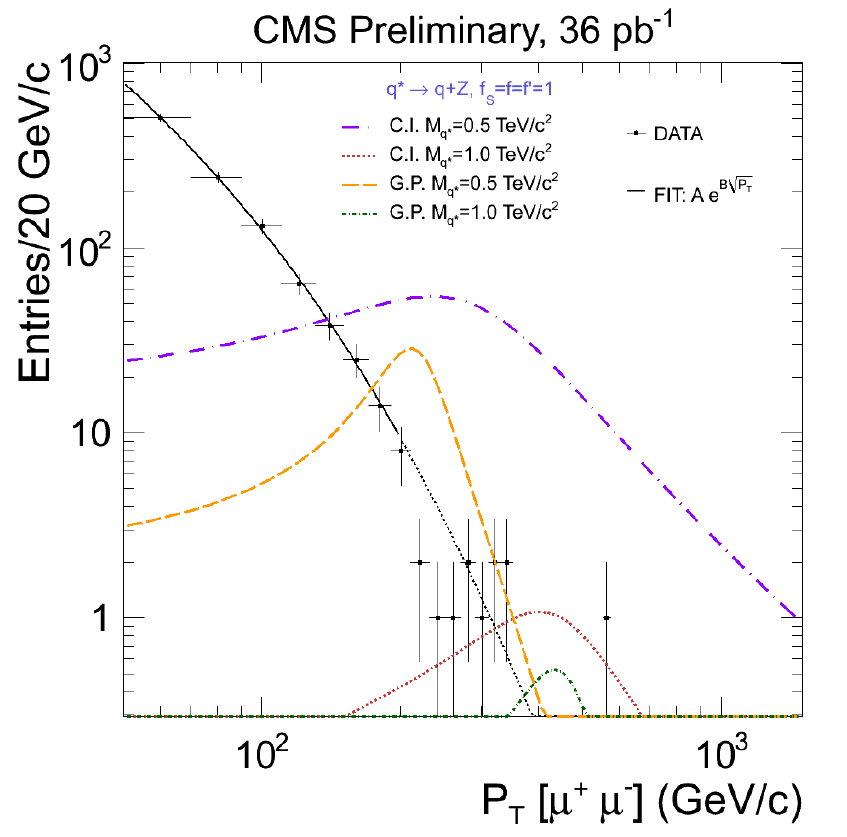
\includegraphics[width=\linewidth]{plots/boosted_z_spectrum.png}

\column{0.33\linewidth}
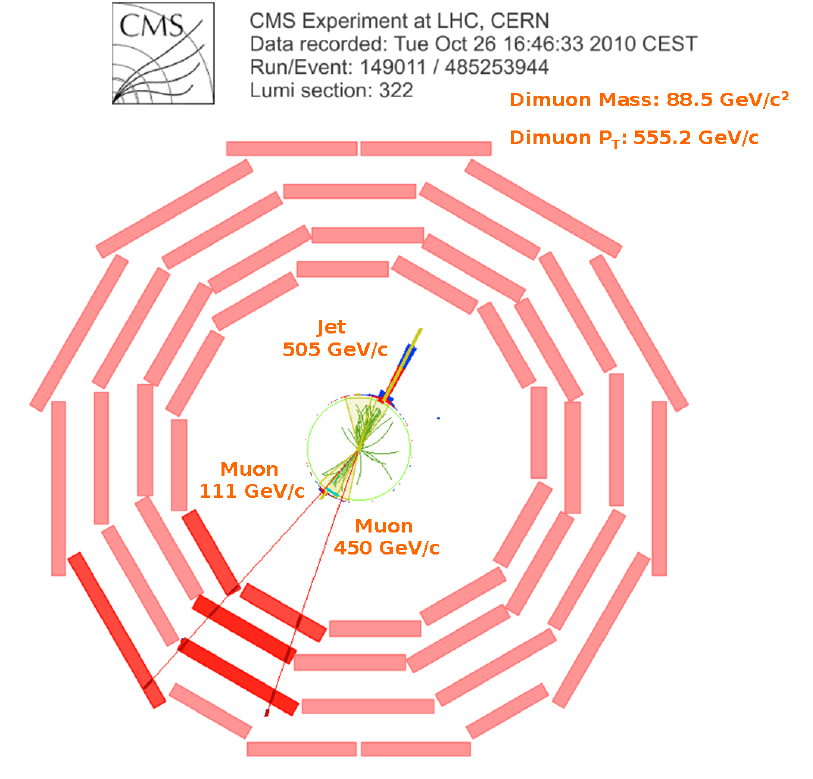
\includegraphics[width=\linewidth]{plots/boosted_z_eventdisplay.png}
\end{columns}

\uncover<2->{\begin{tabular}{c}
\mbox{\hspace{\linewidth}} \\\hline
\end{tabular}

\vspace{0.25 cm}
\mbox{\textcolor{darkblue}{Lepton jets:} one or more low-mass, high-$p_T$ $\gamma_{\scriptsize dark} \to \ell\ell$ from a hidden sector\hspace{-1 cm}}

\vspace{0.25 cm}
\begin{columns}
\column{0.4\linewidth}
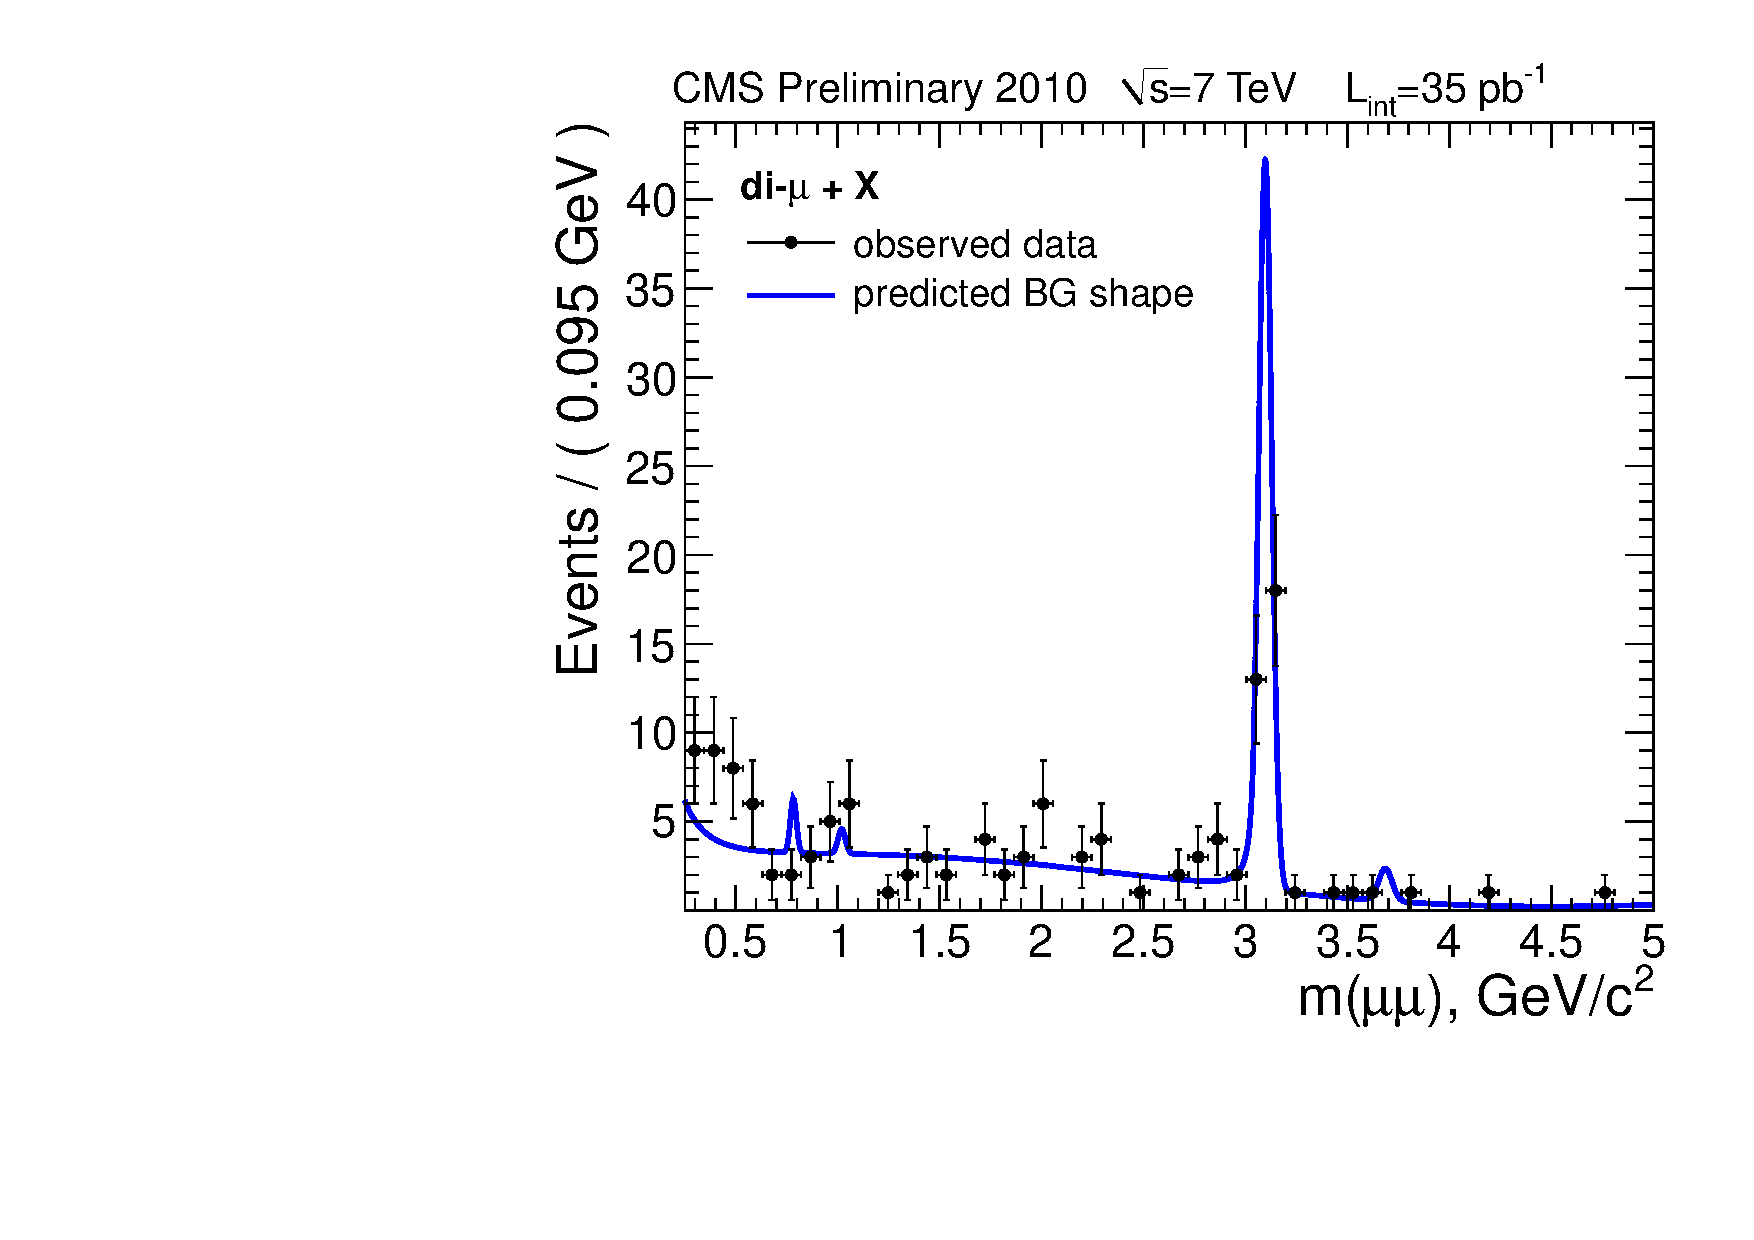
\includegraphics[width=\linewidth]{plots/leptonjets_highpt.pdf}

\column{0.2\linewidth}
Left: high-$p_T$ dimuons

\vspace{0.2 cm}
Right: two dimuons per event

\vspace{0.2 cm}
\textcolor{darkblue}{\scriptsize PAS EXO 11-013}

\column{0.4\linewidth}
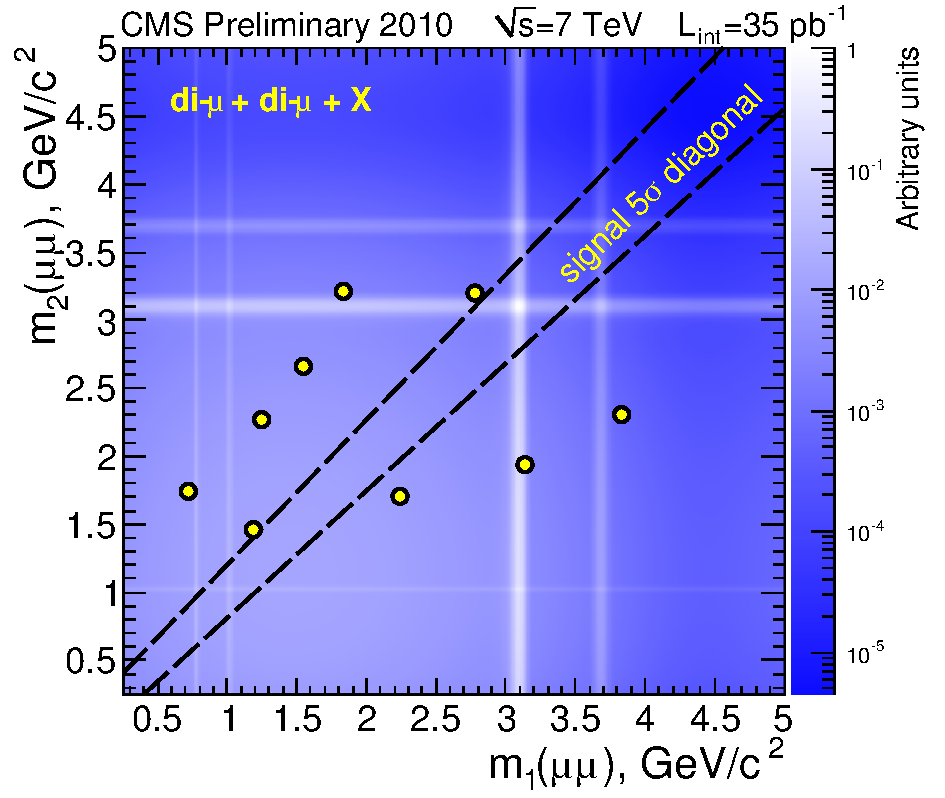
\includegraphics[width=\linewidth]{plots/leptonjets_highmultiplicity.pdf}
\end{columns}}
\end{frame}

\begin{frame}
\frametitle{Diphoton mass spectrum}

\begin{columns}
\column{0.55\linewidth}
\centering $G^*$ resonance simulation \\ \mbox{ }

\column{0.45\linewidth}
\centering data with non-resonant Large Extra Dimensions prediction
\end{columns}

\begin{columns}
\column{0.55\linewidth}
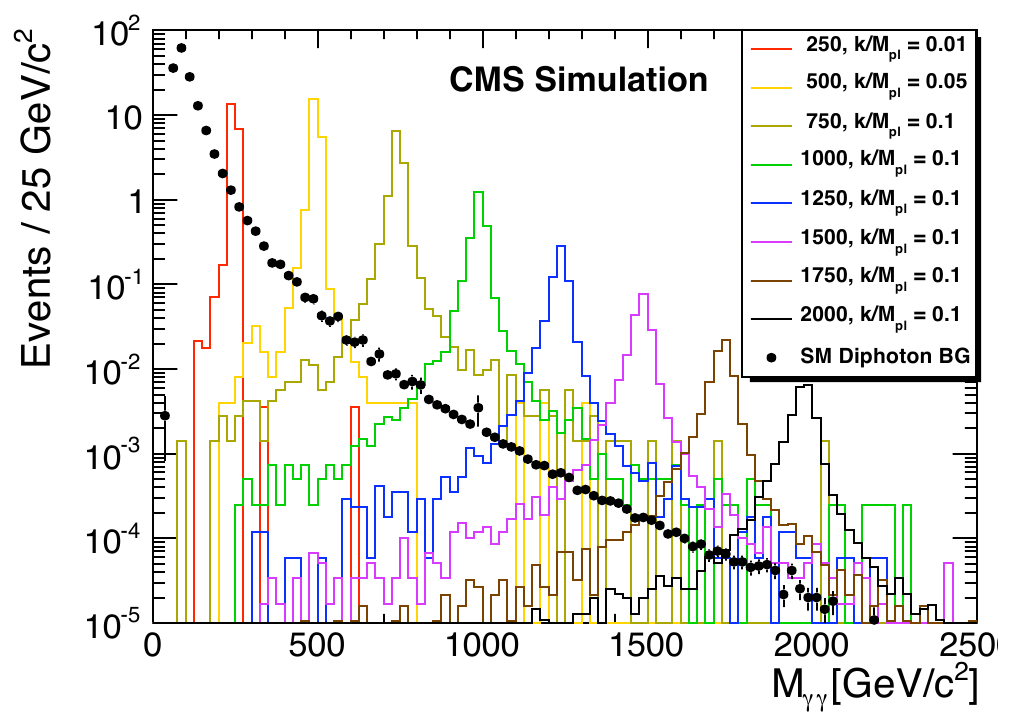
\includegraphics[width=\linewidth]{plots/diphoton_resonant_simulation.png}

\column{0.45\linewidth}
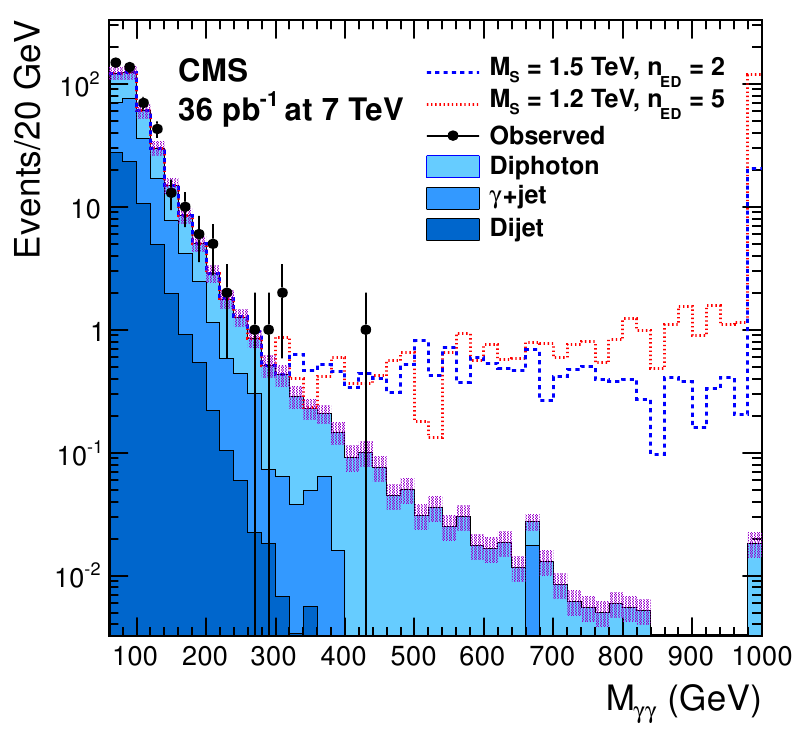
\includegraphics[width=\linewidth]{plots/diphoton_nonresonant_led.png}
\end{columns}

\begin{columns}
\column{0.55\linewidth}
limits with data in \textcolor{darkblue}{\scriptsize PAS EXO 10-019}

\column{0.45\linewidth}
\textcolor{darkblue}{\scriptsize hep-ex/1103.4279}
\end{columns}

%% \vspace{0.75 cm}
%% \hfill
%% \begin{minipage}{0.45\linewidth}
%% Other extra dimensions searches:

%% \vspace{-0.2 cm}
%% \begin{itemize}\setlength{\itemsep}{-0.1 cm}
%% \item monojet + MET \textcolor{darkblue}{\scriptsize EXO 11-003}
%% \item dimuons \textcolor{darkblue}{\scriptsize PAS EXO 10-020}
%% \end{itemize}
%% \end{minipage}
\end{frame}

\begin{frame}
\frametitle{Cross-channels}

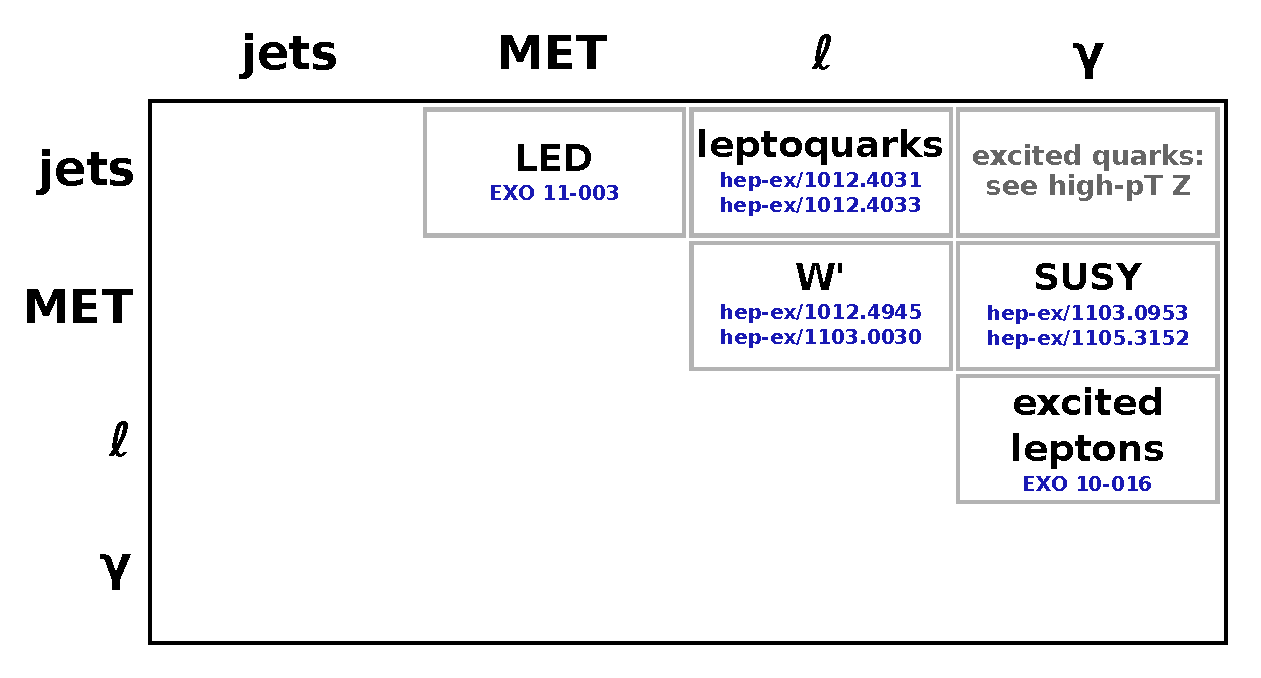
\includegraphics[width=\linewidth]{cross-channels.pdf}

\begin{itemize}
\item<2-> None of the paper references in this talk are repeated
\end{itemize}
\end{frame}

\begin{frame}
\frametitle{Cross-channels: lepton + MET}

\begin{columns}
\column{0.7\linewidth}
Search for $W' \to e\nu$ (left) and $W' \to \mu\nu$ (right) 

\column{0.3\linewidth}
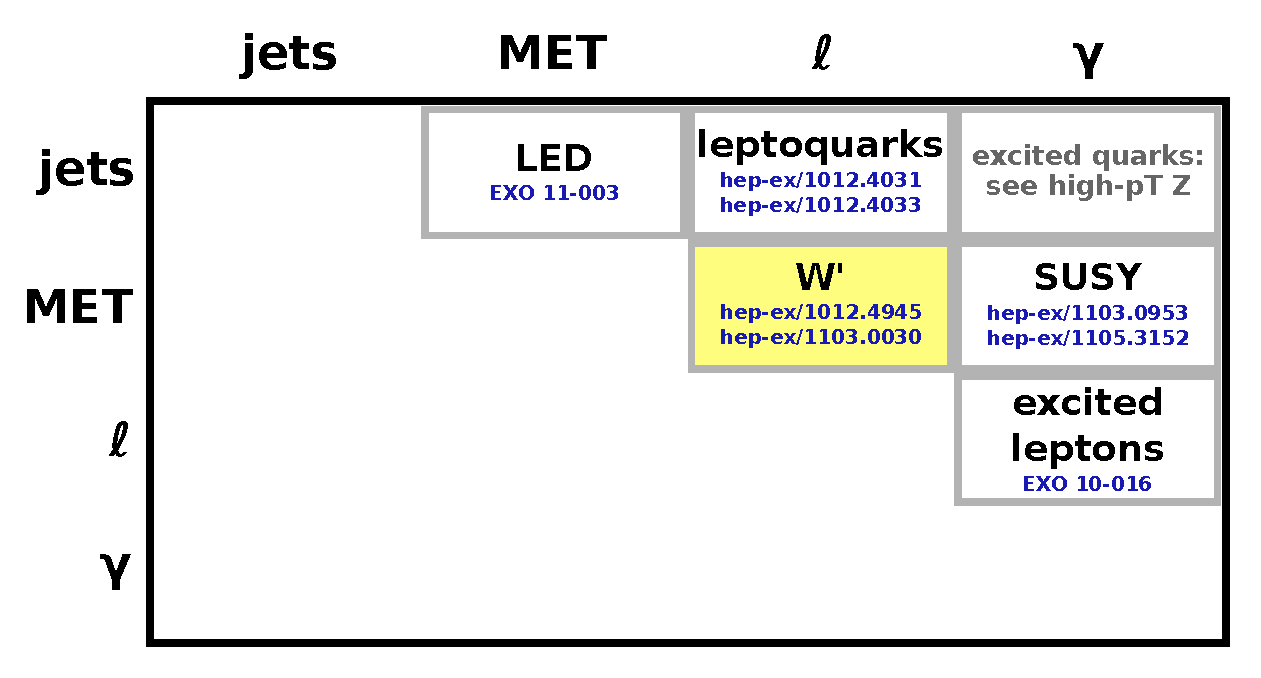
\includegraphics[width=\linewidth]{cross-channels_wprime.pdf}
\end{columns}

\vspace{1 cm}
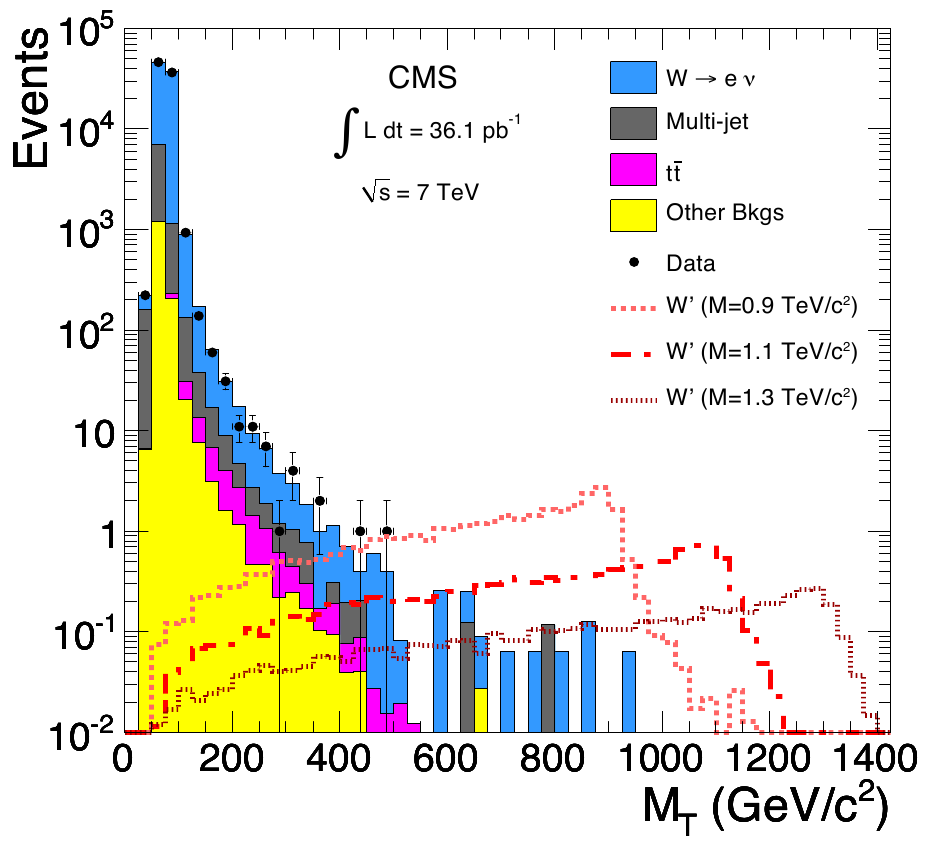
\includegraphics[height=4 cm]{plots/electron_plus_met_mt.png}
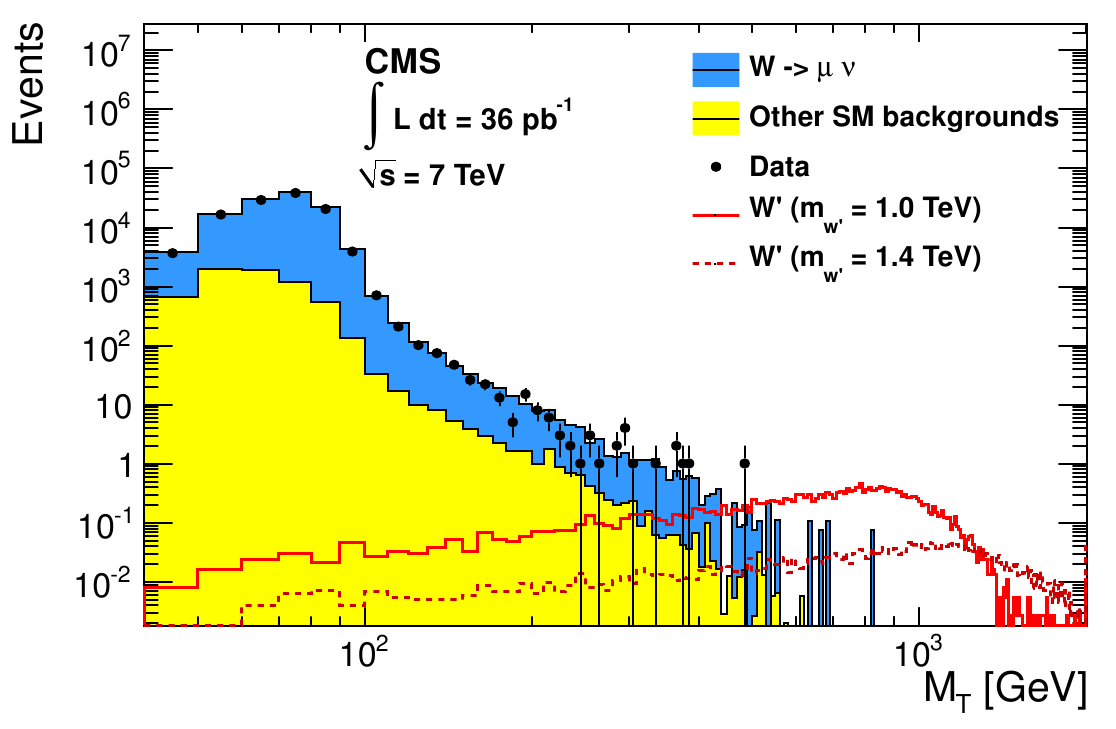
\includegraphics[height=4 cm]{plots/muon_plus_met_mt.png}
\end{frame}

\begin{frame}
\frametitle{Cross-channels: lepton + photon}

\begin{columns}
\column{0.7\linewidth}
Search for $e^* \to e\gamma$ (left) and $\mu^* \to \mu\gamma$ (right) 

\column{0.3\linewidth}
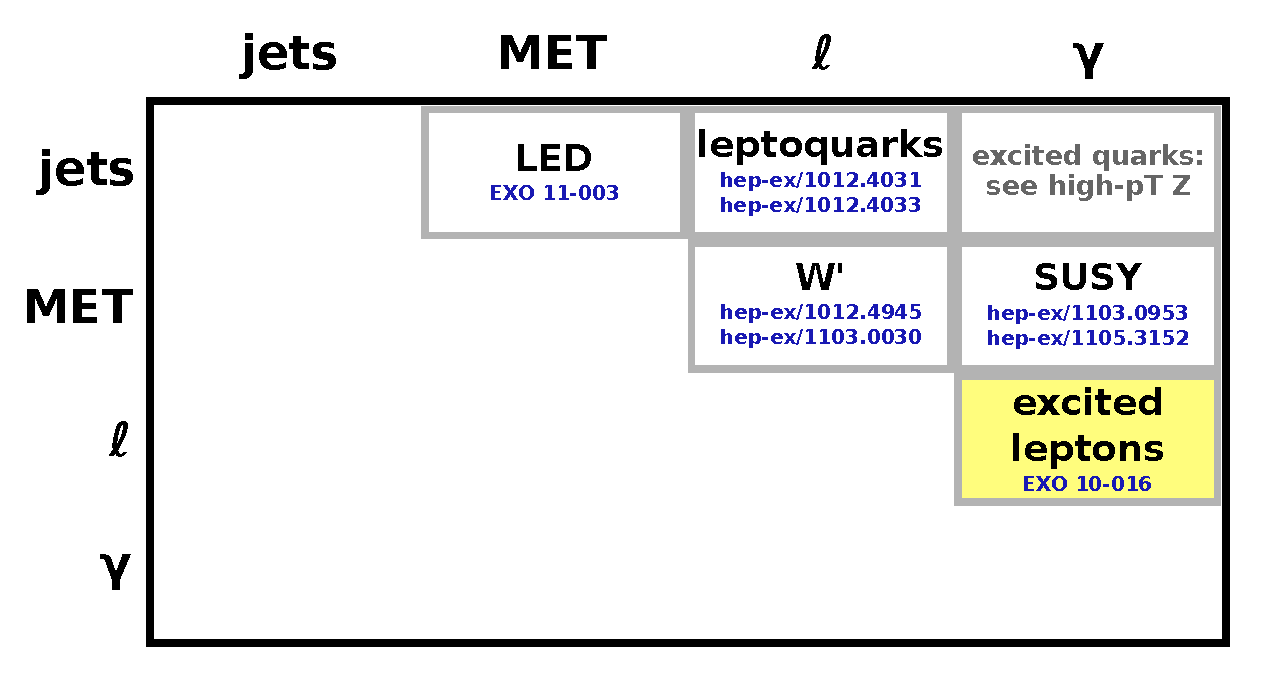
\includegraphics[width=\linewidth]{cross-channels_ellstar.pdf}
\end{columns}

\vspace{1 cm}
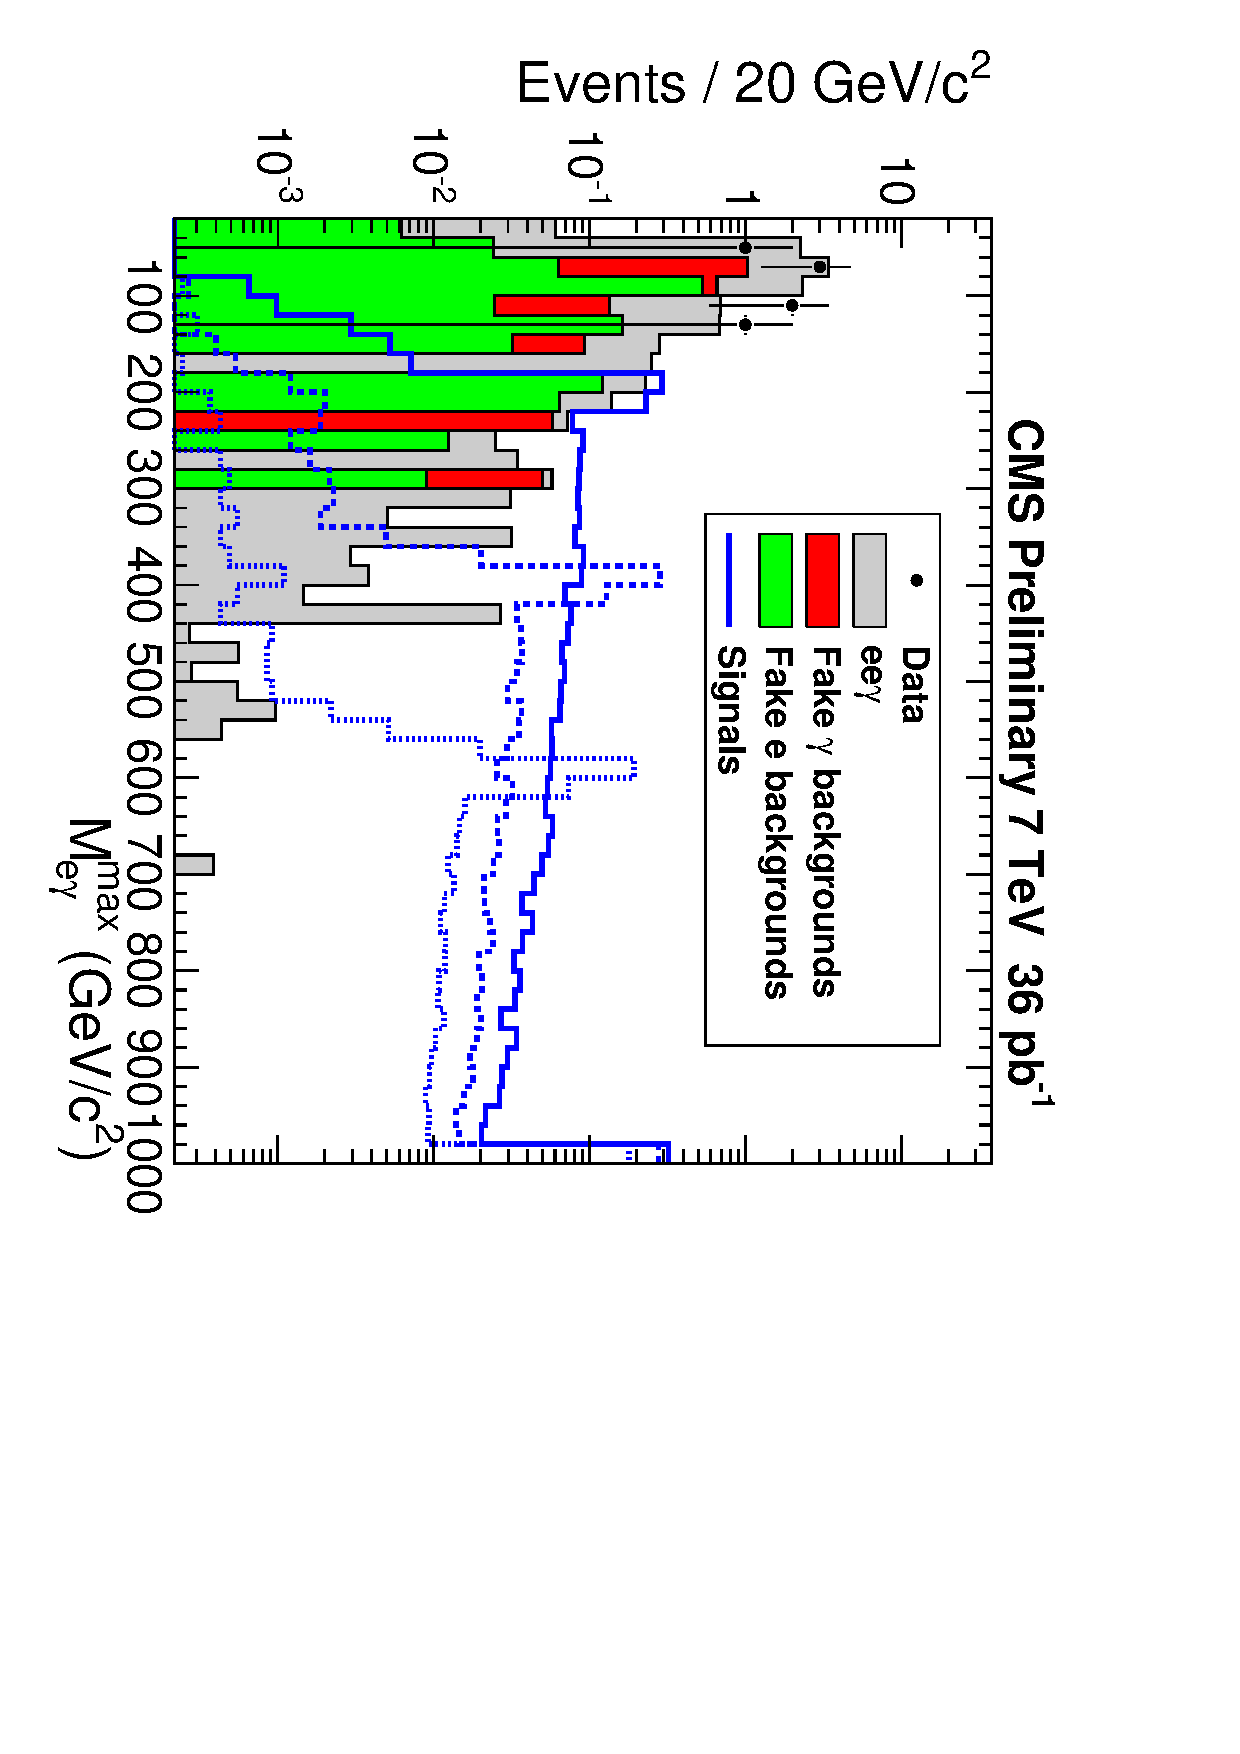
\includegraphics[height=0.5\linewidth, angle=90]{plots/photon_plus_electron.pdf}
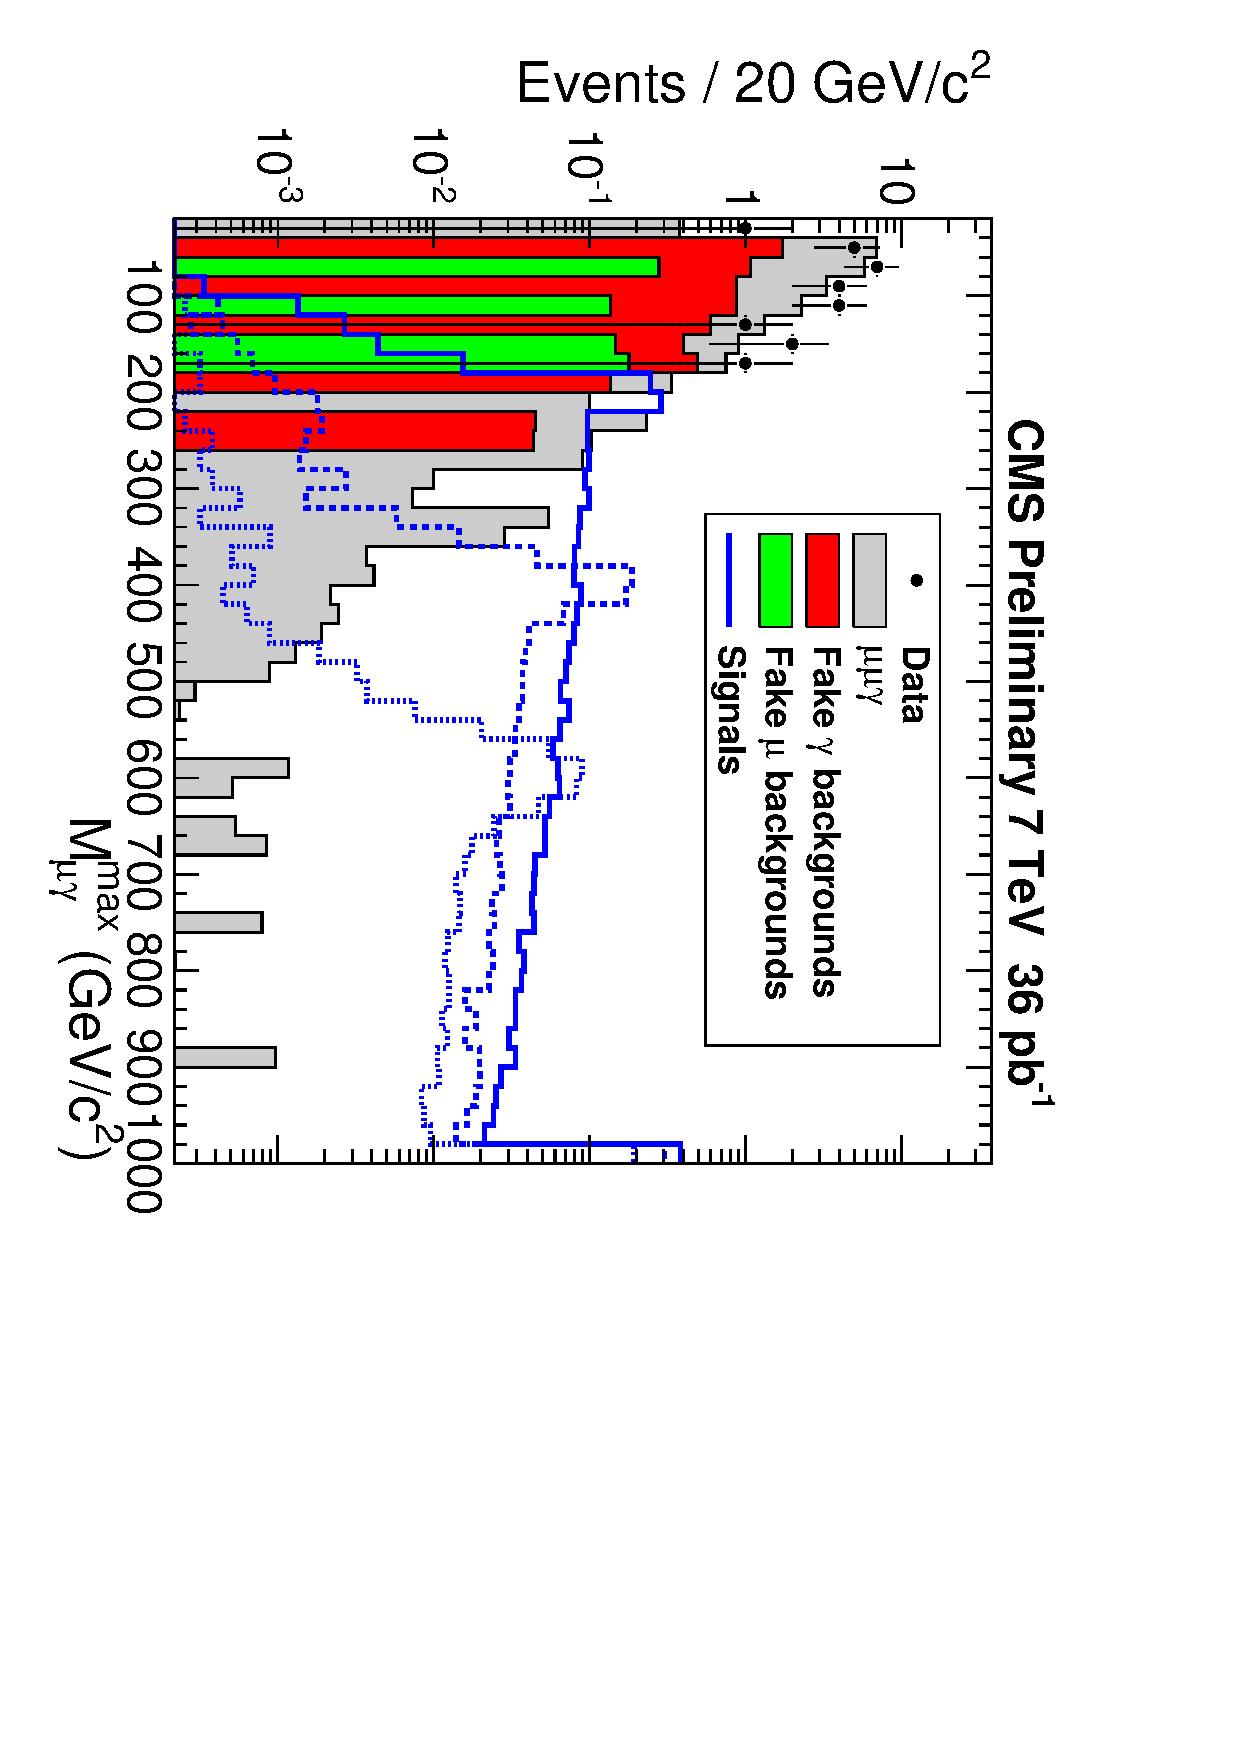
\includegraphics[height=0.5\linewidth, angle=90]{plots/photon_plus_muon.pdf}
\end{frame}

\begin{frame}
\frametitle{Searches using high-level objects}

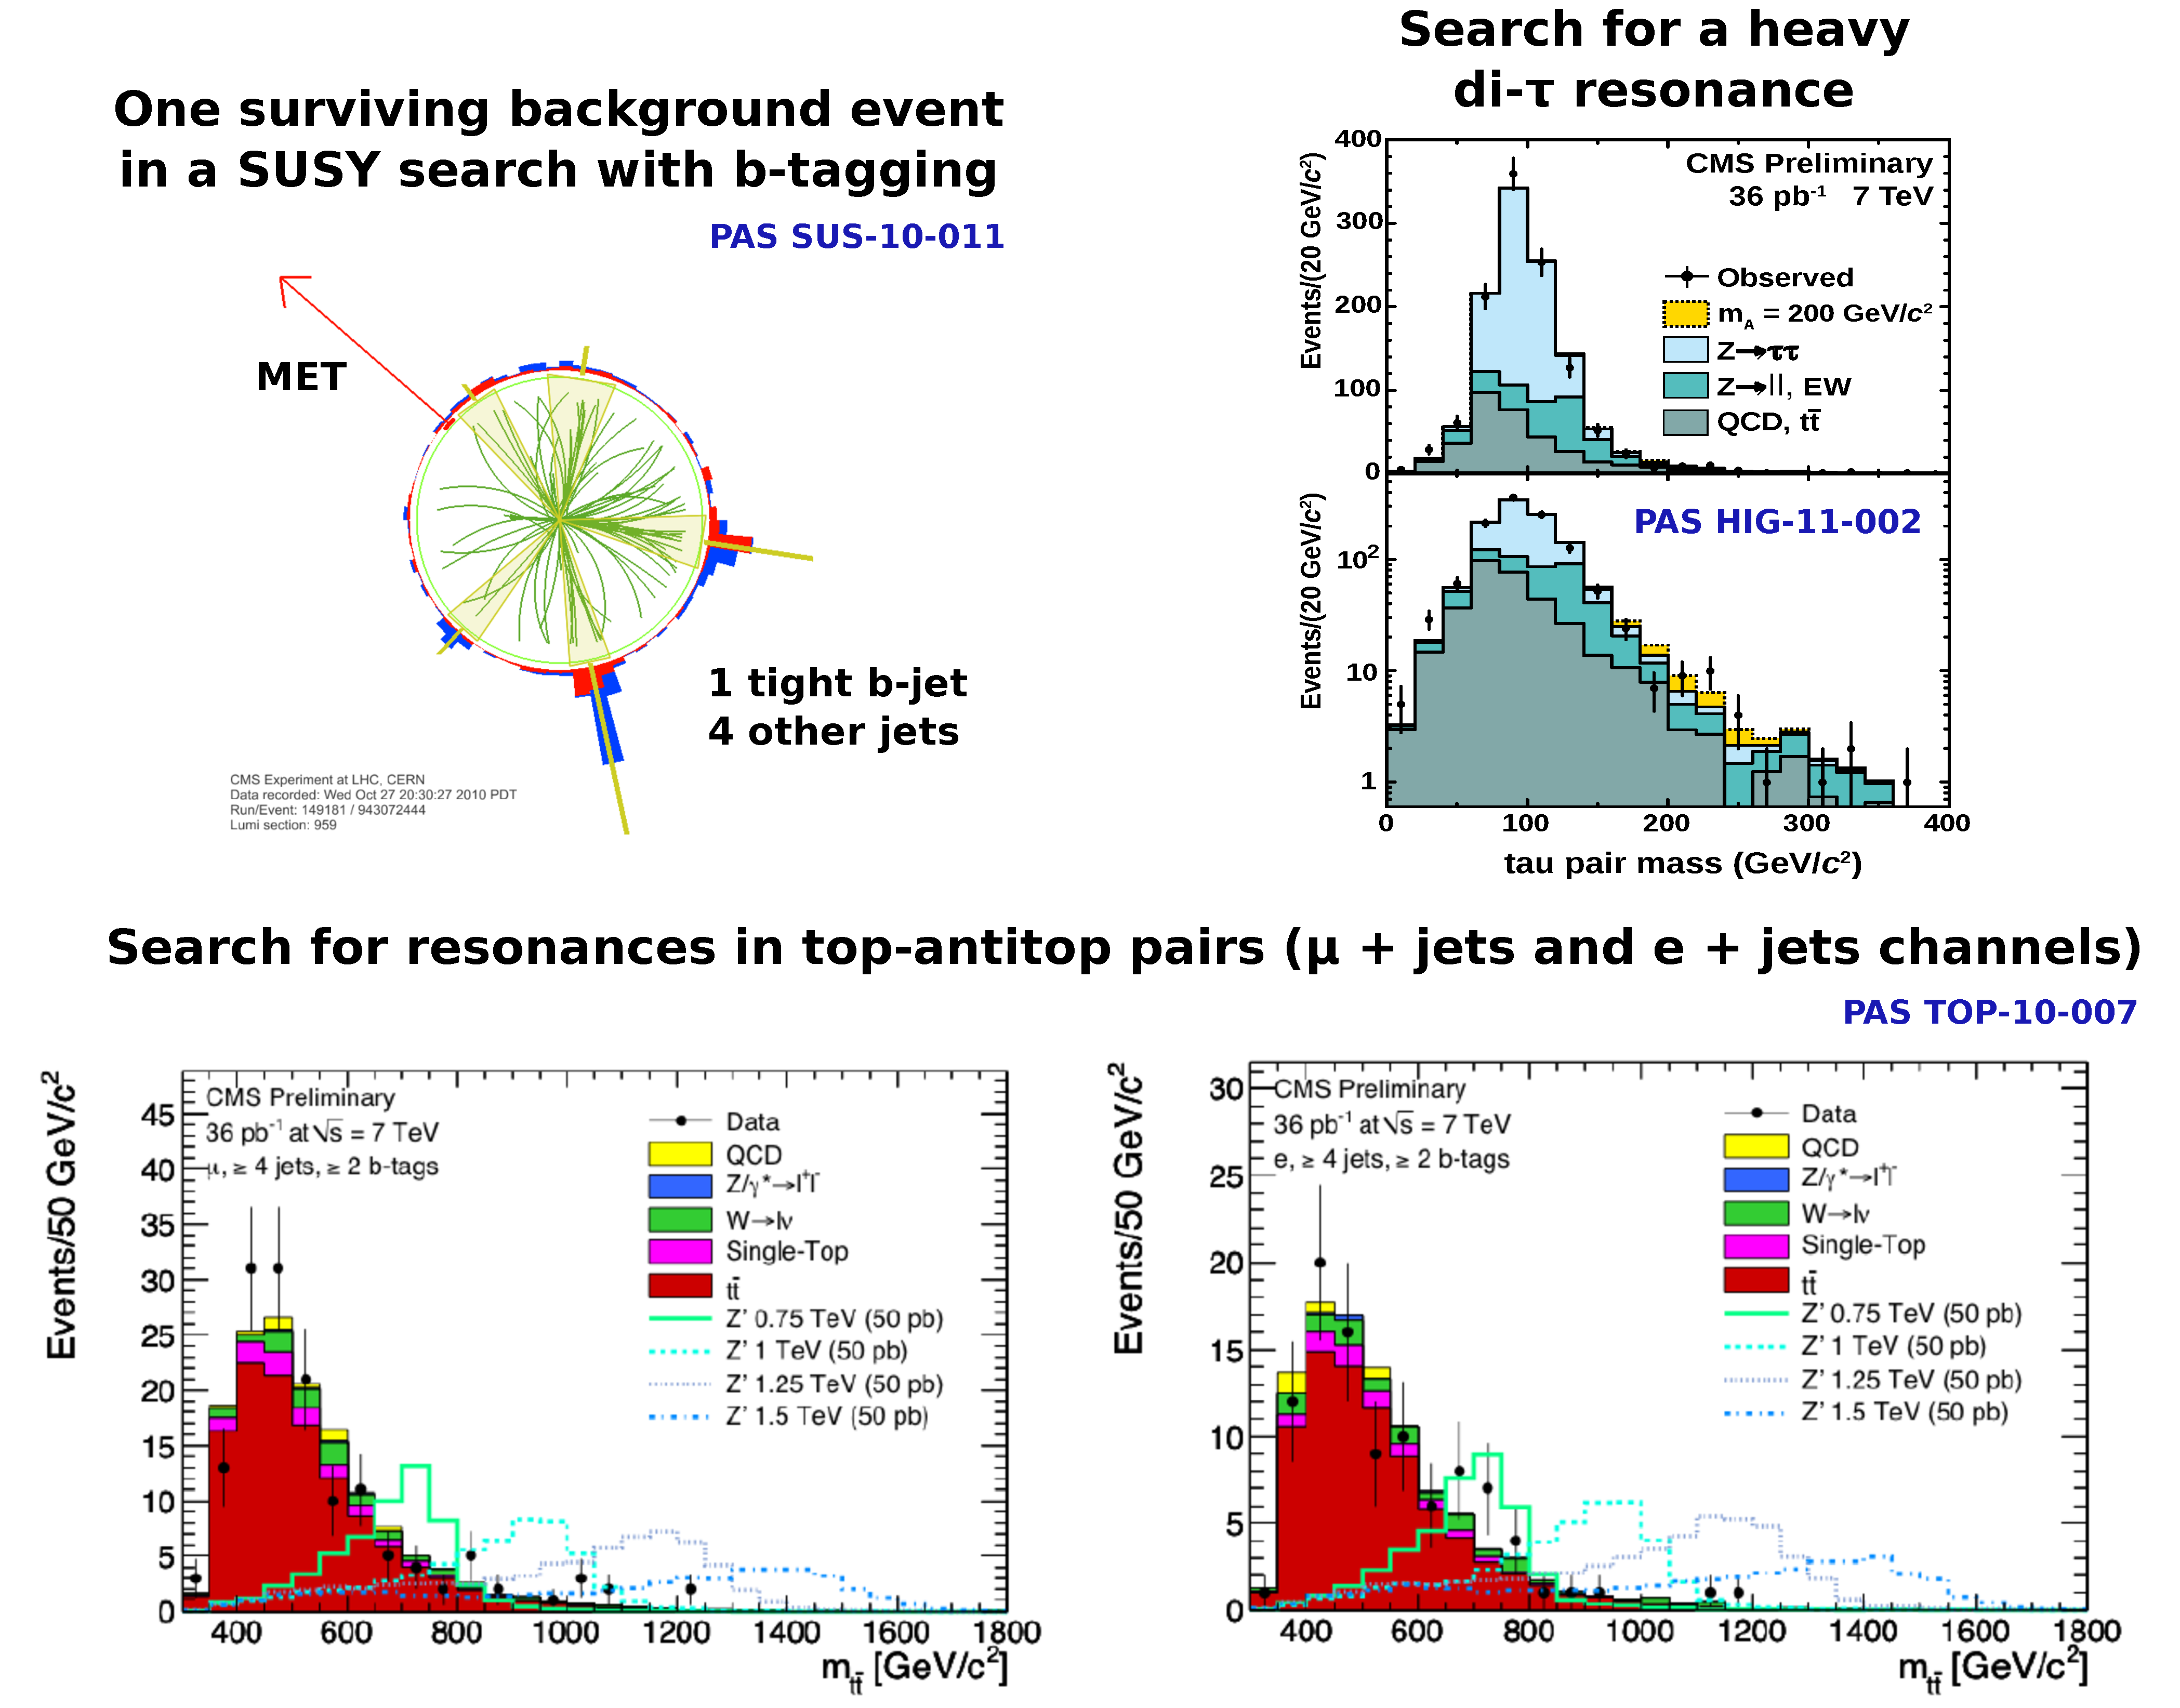
\includegraphics[width=\linewidth]{high-level.pdf}
\end{frame}

\begin{frame}
\frametitle{Microscopic black holes}

\begin{columns}
\column{0.3\linewidth}
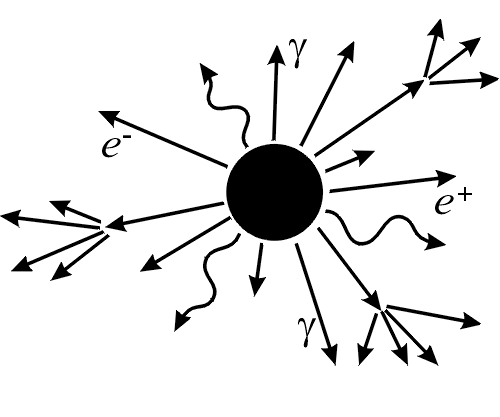
\includegraphics[width=\linewidth]{figures/blackhole_diagram.jpg}

\column{0.7\linewidth}
Extreme cross-channel: high multiplicities of every kind of particle

\vspace{-0.3 cm}
\hfill $\displaystyle S_T = \sum_{E_T > 50\mbox{\scriptsize~GeV}} E_T$ of jets, $e$, $\gamma$, $\mu$

\vspace{0.35 cm}
Set limits on $(4+n)$-D Planck scale $M_D$ (right)
\end{columns}

\vspace{0.35 cm}
\hfill \textcolor{darkblue}{\scriptsize hep-ex/1012.3375}

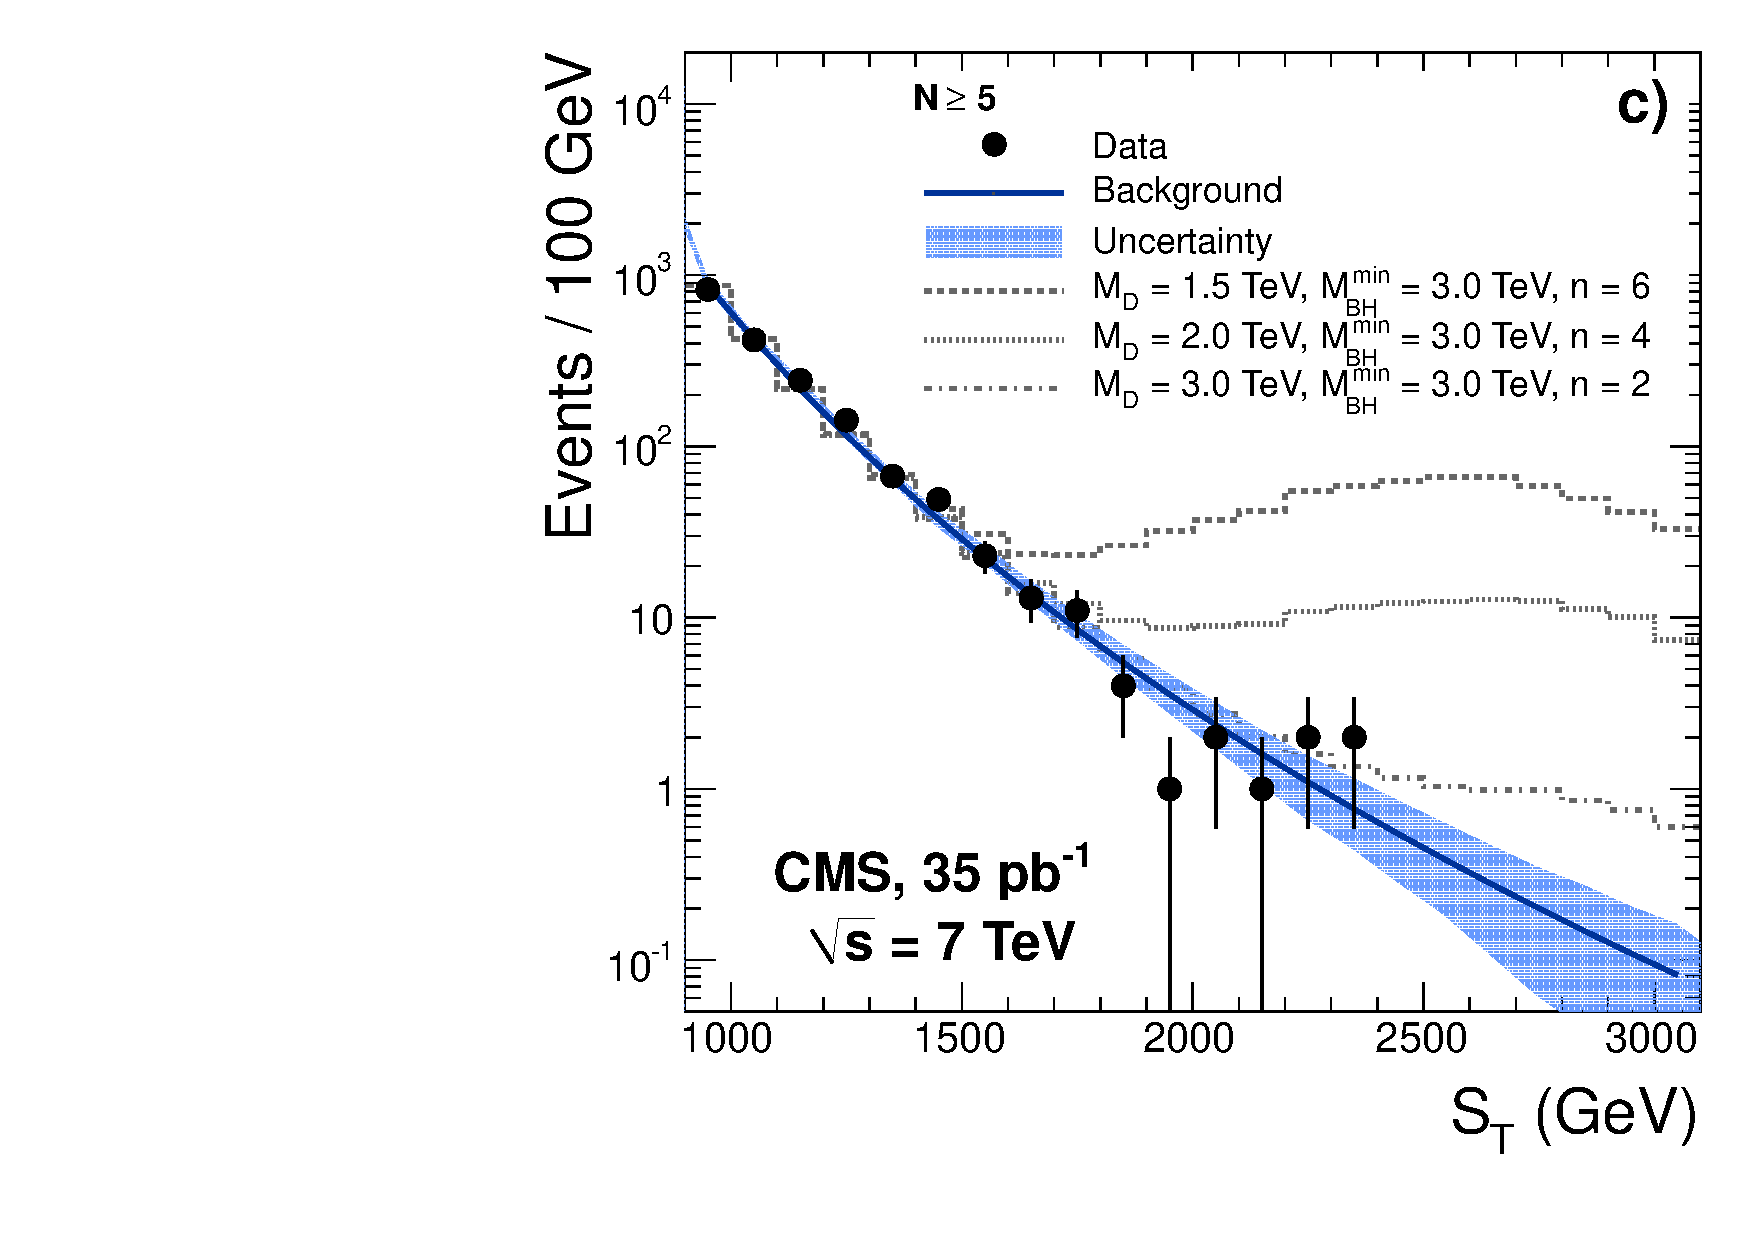
\includegraphics[width=0.45\linewidth]{plots/blackhole_st_5.pdf} \hfill
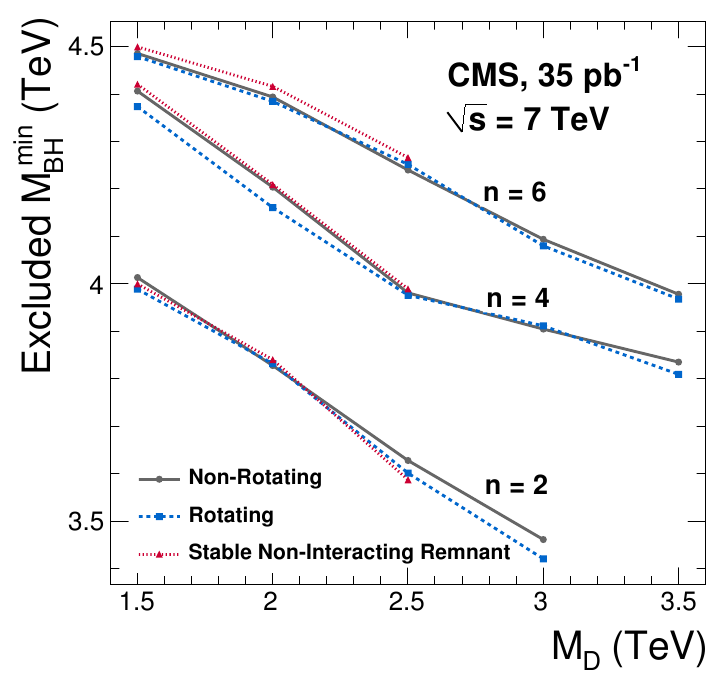
\includegraphics[width=0.45\linewidth]{plots/blackhole_planckscale.png}
\end{frame}

\begin{frame}
\frametitle{Heavy stable charged particles}

\begin{columns}
\column{0.45\linewidth}
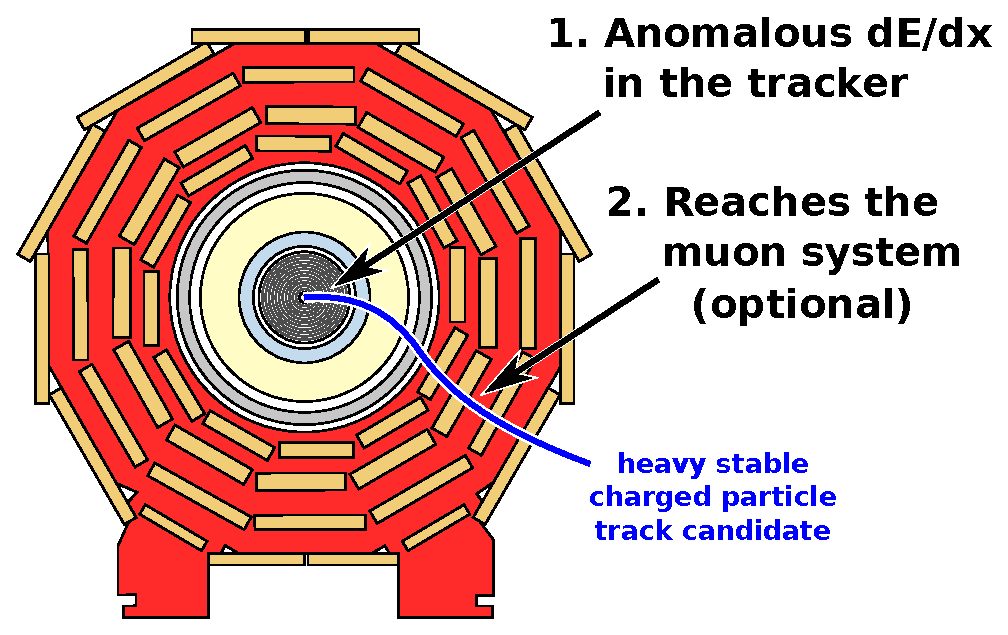
\includegraphics[width=\linewidth]{figures/champ_explanation.pdf}

\column{0.55\linewidth}
Search for anomalously large $dE/dx$ \\ (for $p_T > 15$~GeV/$c$)

\vspace{0.2 cm}
Any particle with $\beta \ll 1$ is BSM

\vspace{0.2 cm}
\mbox{Calculate mass from $dE/dx$ and $|\vec{p}|$\hspace{-1 cm}}
\end{columns}

\hfill \textcolor{darkblue}{\scriptsize hep-ex/1101.1645}

\mbox{ } \hfill 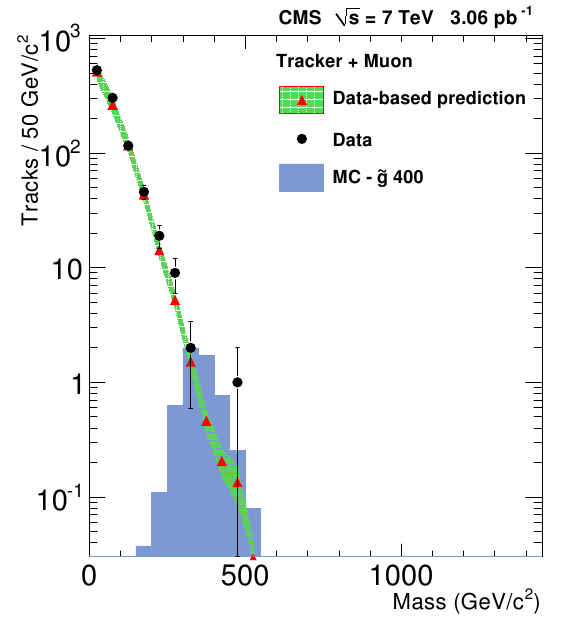
\includegraphics[width=0.4\linewidth]{plots/champ_mass.png} \hfill 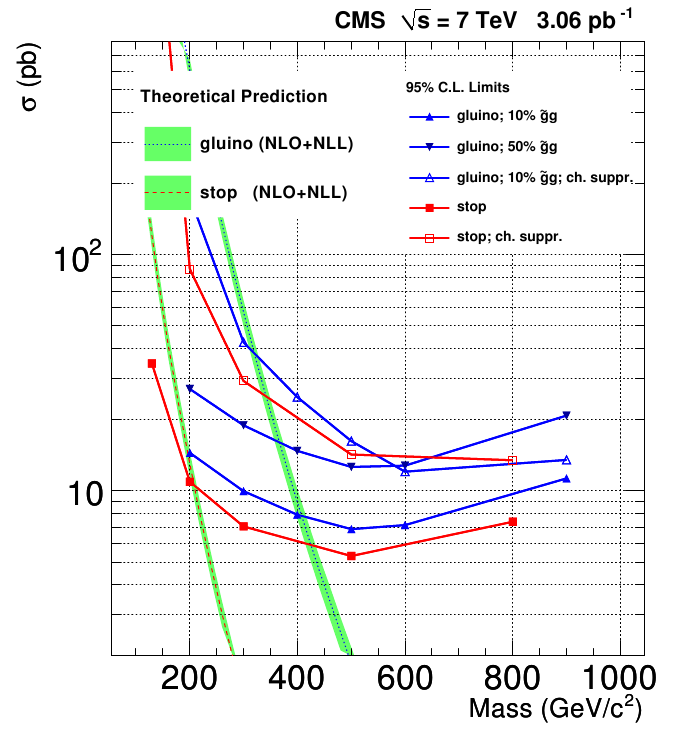
\includegraphics[width=0.4\linewidth]{plots/champ_crosssection.png} \hfill \mbox{ }
\end{frame}

\begin{frame}
\frametitle{Stopped gluinos}

\vspace{2.1 cm}
\hfill \textcolor{darkblue}{\scriptsize hep-ex/1011.5861}

\vspace{-2.6 cm}
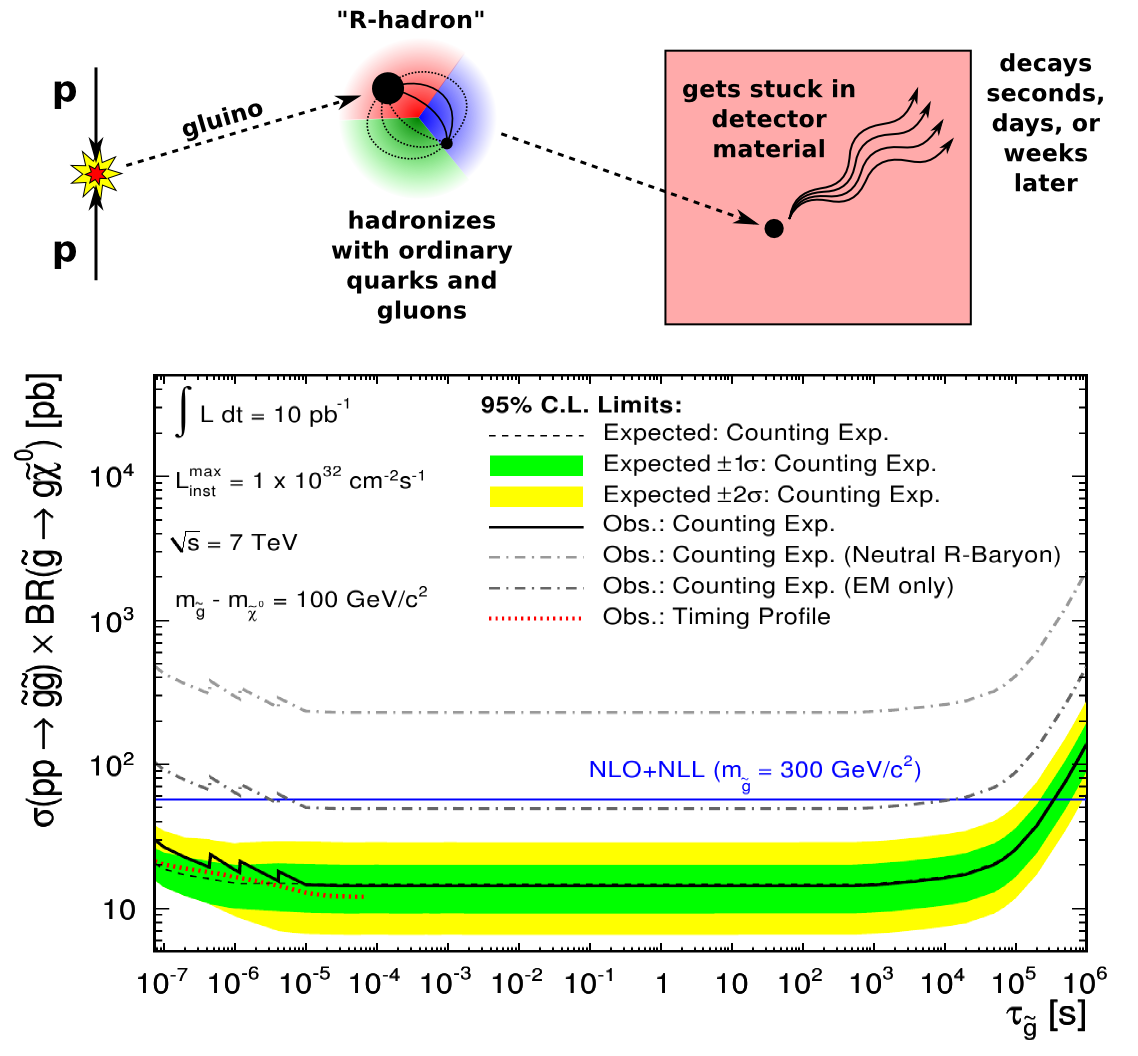
\includegraphics[width=0.85\linewidth]{figures/stoppedgluino.png}
\end{frame}

%% \section*{First section}
%% \begin{frame}
%% \begin{center}
%% \Huge \textcolor{blue}{First section}
%% \end{center}
%% \end{frame}

\begin{frame}
\frametitle{Conclusions}
\begin{itemize}\setlength{\itemsep}{0.5 cm}
\item Broad coverage of experimental signatures: the 2010 data were shaken through a tight sieve, searching for new physics

\item CMS public results

\vspace{0.1 cm}
\mbox{ } \hfill \textcolor{blue}{https://twiki.cern.ch/twiki/bin/view/CMSPublic/PhysicsResults} \hfill \mbox{ }

\item LHC dataset is still growing exponentially: it is reasonable to believe that a dramatic discovery may be in store for us soon
\end{itemize}
\label{numpages}
\end{frame}

\begin{frame}
\frametitle{SUSY limits in the $m_{1/2}$, $m_0$ plane}
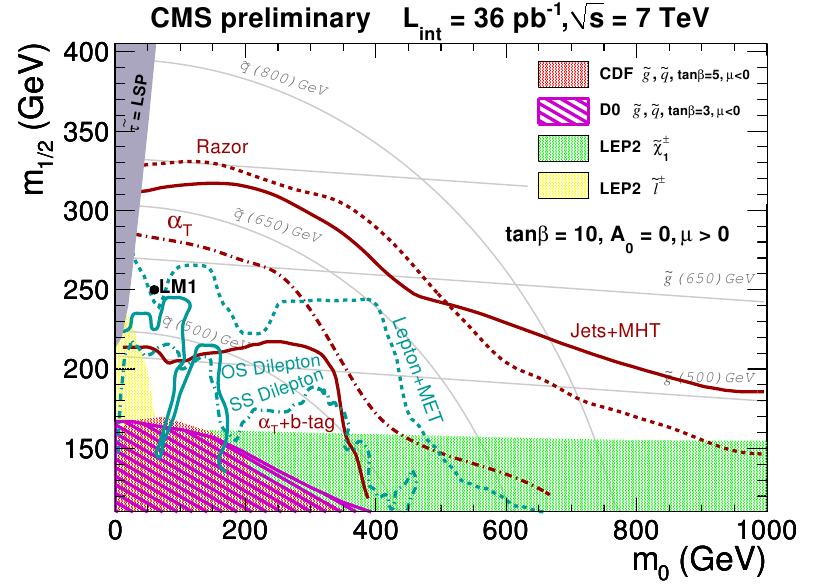
\includegraphics[width=\linewidth]{figures/explicit_models.png}
\end{frame}

\begin{frame}
\frametitle{CMS quarter-view}
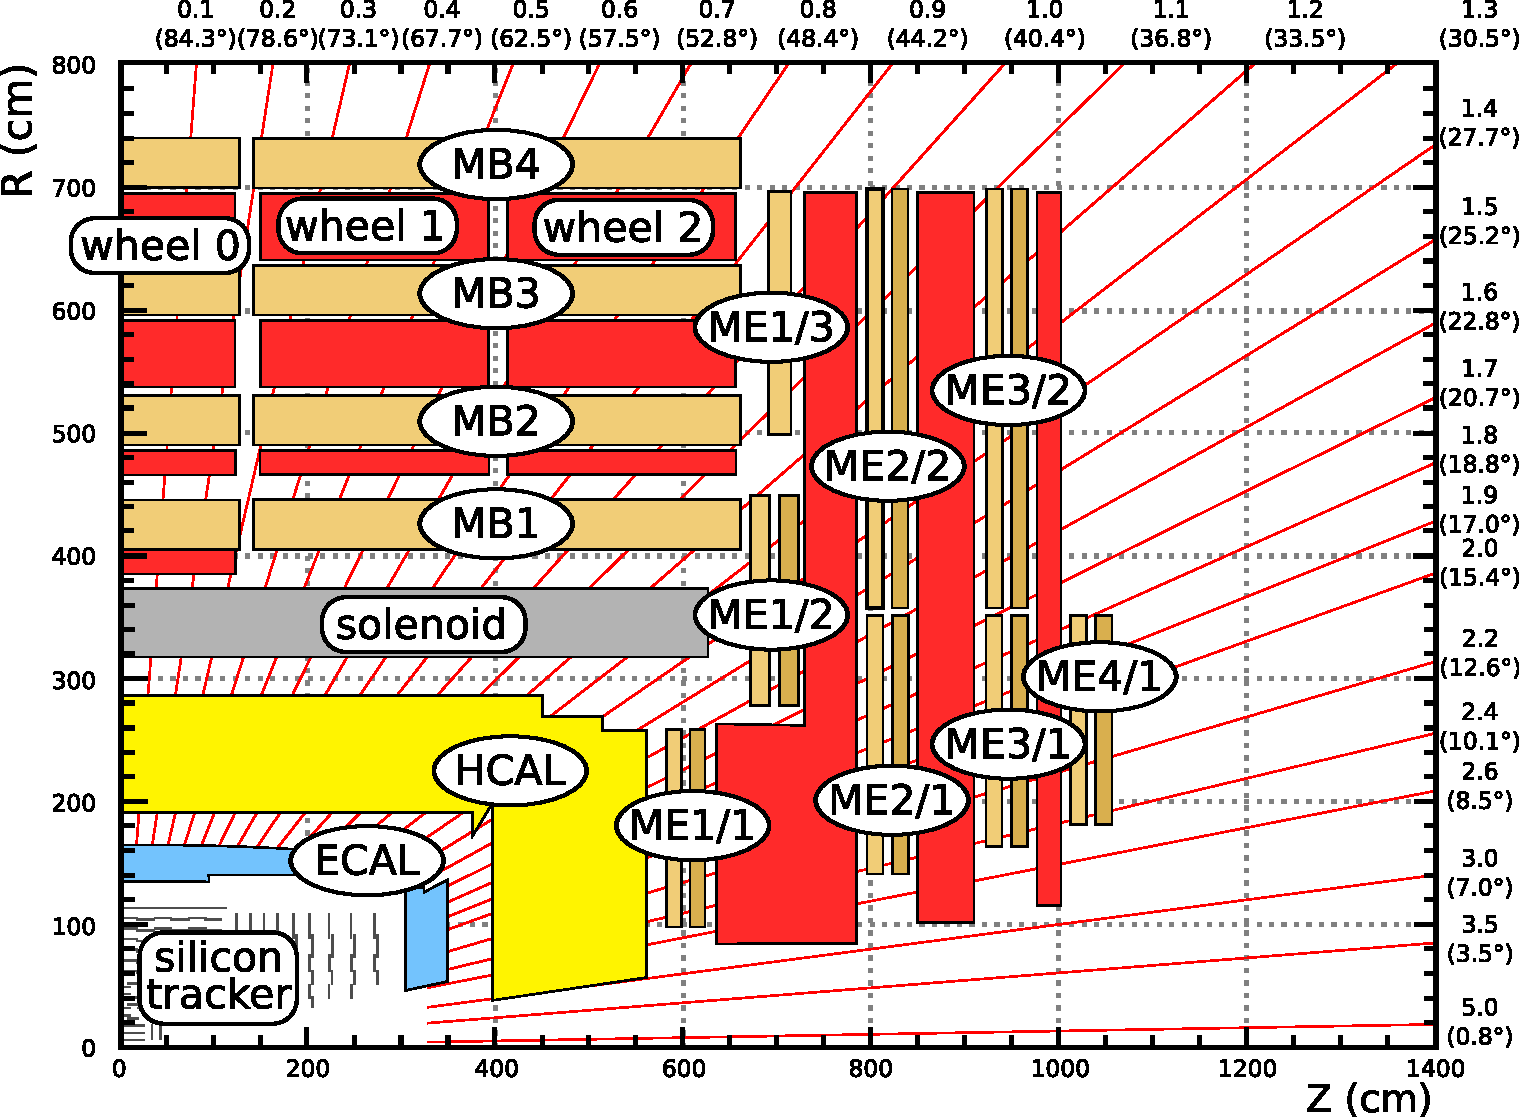
\includegraphics[width=\linewidth]{muon_system_labeled2.pdf}
\end{frame}

\end{document}
